\documentclass[twoside]{book}

% Packages required by doxygen
\usepackage{calc}
\usepackage{doxygen}
\usepackage{graphicx}
\usepackage[utf8]{inputenc}
\usepackage{makeidx}
\usepackage{multicol}
\usepackage{multirow}
\usepackage{fixltx2e}
\PassOptionsToPackage{warn}{textcomp}
\usepackage{textcomp}
\usepackage[nointegrals]{wasysym}
\usepackage[table]{xcolor}

% Font selection
\usepackage[T1]{fontenc}
\usepackage{mathptmx}
\usepackage[scaled=.90]{helvet}
\usepackage{courier}
\usepackage{amssymb}
\usepackage{sectsty}
\renewcommand{\familydefault}{\sfdefault}
\allsectionsfont{%
  \fontseries{bc}\selectfont%
  \color{darkgray}%
}
\renewcommand{\DoxyLabelFont}{%
  \fontseries{bc}\selectfont%
  \color{darkgray}%
}
\newcommand{\+}{\discretionary{\mbox{\scriptsize$\hookleftarrow$}}{}{}}

% Page & text layout
\usepackage{geometry}
\geometry{%
  a4paper,%
  top=2.5cm,%
  bottom=2.5cm,%
  left=2.5cm,%
  right=2.5cm%
}
\tolerance=750
\hfuzz=15pt
\hbadness=750
\setlength{\emergencystretch}{15pt}
\setlength{\parindent}{0cm}
\setlength{\parskip}{0.2cm}
\makeatletter
\renewcommand{\paragraph}{%
  \@startsection{paragraph}{4}{0ex}{-1.0ex}{1.0ex}{%
    \normalfont\normalsize\bfseries\SS@parafont%
  }%
}
\renewcommand{\subparagraph}{%
  \@startsection{subparagraph}{5}{0ex}{-1.0ex}{1.0ex}{%
    \normalfont\normalsize\bfseries\SS@subparafont%
  }%
}
\makeatother

% Headers & footers
\usepackage{fancyhdr}
\pagestyle{fancyplain}
\fancyhead[LE]{\fancyplain{}{\bfseries\thepage}}
\fancyhead[CE]{\fancyplain{}{}}
\fancyhead[RE]{\fancyplain{}{\bfseries\leftmark}}
\fancyhead[LO]{\fancyplain{}{\bfseries\rightmark}}
\fancyhead[CO]{\fancyplain{}{}}
\fancyhead[RO]{\fancyplain{}{\bfseries\thepage}}
\fancyfoot[LE]{\fancyplain{}{}}
\fancyfoot[CE]{\fancyplain{}{}}
\fancyfoot[RE]{\fancyplain{}{\bfseries\scriptsize Generated on Wed Sep 17 2014 09\+:15\+:25 for Phd\+Thesis by Doxygen }}
\fancyfoot[LO]{\fancyplain{}{\bfseries\scriptsize Generated on Wed Sep 17 2014 09\+:15\+:25 for Phd\+Thesis by Doxygen }}
\fancyfoot[CO]{\fancyplain{}{}}
\fancyfoot[RO]{\fancyplain{}{}}
\renewcommand{\footrulewidth}{0.4pt}
\renewcommand{\chaptermark}[1]{%
  \markboth{#1}{}%
}
\renewcommand{\sectionmark}[1]{%
  \markright{\thesection\ #1}%
}

% Indices & bibliography
\usepackage{natbib}
\usepackage[titles]{tocloft}
\setcounter{tocdepth}{3}
\setcounter{secnumdepth}{5}
\makeindex

% Hyperlinks (required, but should be loaded last)
\usepackage{ifpdf}
\ifpdf
  \usepackage[pdftex,pagebackref=true]{hyperref}
\else
  \usepackage[ps2pdf,pagebackref=true]{hyperref}
\fi
\hypersetup{%
  colorlinks=true,%
  linkcolor=blue,%
  citecolor=blue,%
  unicode%
}

% Custom commands
\newcommand{\clearemptydoublepage}{%
  \newpage{\pagestyle{empty}\cleardoublepage}%
}


%===== C O N T E N T S =====

\begin{document}

% Titlepage & ToC
\hypersetup{pageanchor=false,
             bookmarks=true,
             bookmarksnumbered=true,
             pdfencoding=unicode
            }
\pagenumbering{roman}
\begin{titlepage}
\vspace*{7cm}
\begin{center}%
{\Large Phd\+Thesis }\\
\vspace*{1cm}
{\large Generated by Doxygen 1.8.7}\\
\vspace*{0.5cm}
{\small Wed Sep 17 2014 09:15:25}\\
\end{center}
\end{titlepage}
\clearemptydoublepage
\tableofcontents
\clearemptydoublepage
\pagenumbering{arabic}
\hypersetup{pageanchor=true}

%--- Begin generated contents ---
\chapter{Class Index}
\section{Class List}
Here are the classes, structs, unions and interfaces with brief descriptions\+:\begin{DoxyCompactList}
\item\contentsline{section}{\hyperlink{class_area_feature_extractor}{Area\+Feature\+Extractor} }{\pageref{class_area_feature_extractor}}{}
\item\contentsline{section}{\hyperlink{class_complex_network}{Complex\+Network$<$ N\+O\+D\+E\+\_\+\+T\+Y\+P\+E, E\+D\+G\+E\+\_\+\+T\+Y\+P\+E $>$} \\*Rede Complexa }{\pageref{class_complex_network}}{}
\item\contentsline{section}{\hyperlink{class_complex_network_constructor}{Complex\+Network\+Constructor} }{\pageref{class_complex_network_constructor}}{}
\item\contentsline{section}{\hyperlink{class_database_reader}{Database\+Reader} }{\pageref{class_database_reader}}{}
\item\contentsline{section}{\hyperlink{class_edge}{Edge$<$ N\+O\+D\+E\+\_\+\+T\+Y\+P\+E, E\+D\+G\+E\+\_\+\+T\+Y\+P\+E $>$} }{\pageref{class_edge}}{}
\item\contentsline{section}{\hyperlink{class_feature}{Feature} }{\pageref{class_feature}}{}
\item\contentsline{section}{\hyperlink{class_feature_extractor}{Feature\+Extractor} }{\pageref{class_feature_extractor}}{}
\item\contentsline{section}{\hyperlink{class_link}{Link} }{\pageref{class_link}}{}
\item\contentsline{section}{\hyperlink{class_node}{Node$<$ N\+O\+D\+E\+\_\+\+T\+Y\+P\+E, E\+D\+G\+E\+\_\+\+T\+Y\+P\+E $>$} }{\pageref{class_node}}{}
\item\contentsline{section}{\hyperlink{classnode__t}{node\+\_\+t} }{\pageref{classnode__t}}{}
\item\contentsline{section}{\hyperlink{class_region}{Region} }{\pageref{class_region}}{}
\item\contentsline{section}{\hyperlink{class_sun_database_reader}{Sun\+Database\+Reader} }{\pageref{class_sun_database_reader}}{}
\item\contentsline{section}{\hyperlink{class_supervised_image}{Supervised\+Image} }{\pageref{class_supervised_image}}{}
\end{DoxyCompactList}

\chapter{File Index}
\section{File List}
Here is a list of all files with brief descriptions\+:\begin{DoxyCompactList}
\item\contentsline{section}{src/\hyperlink{_complex_network_8cpp}{Complex\+Network.\+cpp} }{\pageref{_complex_network_8cpp}}{}
\item\contentsline{section}{src/\hyperlink{_complex_network_8hpp}{Complex\+Network.\+hpp} }{\pageref{_complex_network_8hpp}}{}
\item\contentsline{section}{src/\hyperlink{_edge_8cpp}{Edge.\+cpp} }{\pageref{_edge_8cpp}}{}
\item\contentsline{section}{src/\hyperlink{_edge_8hpp}{Edge.\+hpp} }{\pageref{_edge_8hpp}}{}
\item\contentsline{section}{src/\hyperlink{main_8cpp}{main.\+cpp} }{\pageref{main_8cpp}}{}
\item\contentsline{section}{src/\hyperlink{_node_8cpp}{Node.\+cpp} }{\pageref{_node_8cpp}}{}
\item\contentsline{section}{src/\hyperlink{_node_8hpp}{Node.\+hpp} }{\pageref{_node_8hpp}}{}
\end{DoxyCompactList}

\chapter{Class Documentation}
\hypertarget{class_complex_network}{\section{Complex\+Network$<$ N\+O\+D\+E\+\_\+\+T\+Y\+P\+E, E\+D\+G\+E\+\_\+\+T\+Y\+P\+E $>$ Class Template Reference}
\label{class_complex_network}\index{Complex\+Network$<$ N\+O\+D\+E\+\_\+\+T\+Y\+P\+E, E\+D\+G\+E\+\_\+\+T\+Y\+P\+E $>$@{Complex\+Network$<$ N\+O\+D\+E\+\_\+\+T\+Y\+P\+E, E\+D\+G\+E\+\_\+\+T\+Y\+P\+E $>$}}
}


{\ttfamily \#include $<$Complex\+Network.\+hpp$>$}

\subsection*{Classes}
\begin{DoxyCompactItemize}
\item 
class \hyperlink{class_complex_network_1_1_edge_iterator}{Edge\+Iterator}
\item 
class \hyperlink{class_complex_network_1_1_node_iterator}{Node\+Iterator}
\end{DoxyCompactItemize}
\subsection*{Public Member Functions}
\begin{DoxyCompactItemize}
\item 
\hyperlink{class_complex_network_a4a16e825e1d8b487067ca21d677617a3}{Complex\+Network} (bool \hyperlink{class_complex_network_ae1f8a32f89d84aab42475d8fe46dfa09}{directed}=true)
\item 
virtual \hyperlink{_complex_network_8hpp_a8323334ca788fde39682469321590d52}{node\+\_\+id} \hyperlink{class_complex_network_af2c31ca0d2142dafa1d88ca3ff22356f}{add\+Node} (const N\+O\+D\+E\+\_\+\+T\+Y\+P\+E \&n)
\item 
virtual N\+O\+D\+E\+\_\+\+T\+Y\+P\+E $\ast$ \hyperlink{class_complex_network_a3711aff250a942a9ad61d0571be82c43}{get\+Node} (\hyperlink{_complex_network_8hpp_a8323334ca788fde39682469321590d52}{node\+\_\+id} id)
\item 
virtual bool \hyperlink{class_complex_network_a33f2b4528cc31296ede98be7e6dcd600}{remove\+Node} (\hyperlink{_complex_network_8hpp_a8323334ca788fde39682469321590d52}{node\+\_\+id} id)
\item 
virtual void \hyperlink{class_complex_network_a52c25eb9c9c642a39681e4040fc0a17d}{add\+Edge} (\hyperlink{_complex_network_8hpp_a8323334ca788fde39682469321590d52}{node\+\_\+id} from, \hyperlink{_complex_network_8hpp_a8323334ca788fde39682469321590d52}{node\+\_\+id} to, const E\+D\+G\+E\+\_\+\+T\+Y\+P\+E \&e)
\item 
virtual E\+D\+G\+E\+\_\+\+T\+Y\+P\+E $\ast$ \hyperlink{class_complex_network_a6a1c638e4604efe06c12ce3065020ec1}{get\+Edge} (\hyperlink{_complex_network_8hpp_a8323334ca788fde39682469321590d52}{node\+\_\+id} from, \hyperlink{_complex_network_8hpp_a8323334ca788fde39682469321590d52}{node\+\_\+id} to)
\item 
virtual E\+D\+G\+E\+\_\+\+T\+Y\+P\+E $\ast$ \hyperlink{class_complex_network_ad440008416fc33500754d77b2532560f}{get\+Edge\+From\+Edge\+Id} (\hyperlink{_complex_network_8hpp_ad7d18d7b90a45b6625704e92d10aa3a0}{edge\+\_\+id} id)
\item 
virtual bool \hyperlink{class_complex_network_a9b2c7df561a2ad5fc14b04a5c5c56828}{remove\+Edge} (\hyperlink{_complex_network_8hpp_a8323334ca788fde39682469321590d52}{node\+\_\+id} from, \hyperlink{_complex_network_8hpp_a8323334ca788fde39682469321590d52}{node\+\_\+id} to)
\item 
virtual void \hyperlink{class_complex_network_a64db5949375a84eba3d9ff559d68fc6e}{clear} ()
\item 
unsigned int \hyperlink{class_complex_network_afee98f26ceed674c17be01a740787170}{get\+Num\+Nodes} () const 
\item 
unsigned int \hyperlink{class_complex_network_a720cb4e40342648d394792cc693d29a5}{get\+Num\+Edges} () const 
\item 
\hyperlink{class_complex_network_1_1_node_iterator}{Node\+Iterator} \hyperlink{class_complex_network_ab02bc6912437322f146f6ce98b415759}{Begin} ()
\item 
\hyperlink{class_complex_network_1_1_node_iterator}{Node\+Iterator} \hyperlink{class_complex_network_a2c90f4efd046776d7a53776b24daae0f}{End} ()
\item 
\hyperlink{class_complex_network_1_1_edge_iterator}{Edge\+Iterator} \hyperlink{class_complex_network_a2167b224079f5c0b44443959ad0b6440}{Edges\+Begin} (\hyperlink{_complex_network_8hpp_a8323334ca788fde39682469321590d52}{node\+\_\+id} node\+\_\+from)
\item 
\hyperlink{class_complex_network_1_1_edge_iterator}{Edge\+Iterator} \hyperlink{class_complex_network_ad806138ea94ec18ed17f4681ab731208}{Edges\+End} (\hyperlink{_complex_network_8hpp_a8323334ca788fde39682469321590d52}{node\+\_\+id} node\+\_\+from)
\item 
\hyperlink{class_complex_network_1_1_edge_iterator}{Edge\+Iterator} \hyperlink{class_complex_network_a3a228b9a9497db2b9385deb4eb39f1e1}{Edges\+Begin} ()
\item 
\hyperlink{class_complex_network_1_1_edge_iterator}{Edge\+Iterator} \hyperlink{class_complex_network_afa7d628b66a815d97afbf5373640d12b}{Edges\+End} ()
\item 
unsigned int \hyperlink{class_complex_network_a4036d2cda2dc5596d03e164c3455aff6}{get\+Num\+Edges} (\hyperlink{_complex_network_8hpp_a8323334ca788fde39682469321590d52}{node\+\_\+id}) const 
\item 
void \hyperlink{class_complex_network_a5d127d4296808b7ccdadccaa58084e96}{save} (const char $\ast$filename)
\item 
void \hyperlink{class_complex_network_a54fbdb35418f424e8dad0dbc5dc16bee}{load} (const char $\ast$filename)
\item 
\hyperlink{class_complex_network}{Complex\+Network}$<$ N\+O\+D\+E\+\_\+\+T\+Y\+P\+E, \\*
E\+D\+G\+E\+\_\+\+T\+Y\+P\+E $>$ \& \hyperlink{class_complex_network_a5a8b07f5ca5d247e13a2e2bc5ac75de1}{operator=} (const \hyperlink{class_complex_network}{Complex\+Network}$<$ N\+O\+D\+E\+\_\+\+T\+Y\+P\+E, E\+D\+G\+E\+\_\+\+T\+Y\+P\+E $>$ \&cn)
\end{DoxyCompactItemize}
\subsection*{Protected Member Functions}
\begin{DoxyCompactItemize}
\item 
Q\+Pair$<$ \hyperlink{_complex_network_8hpp_a8323334ca788fde39682469321590d52}{node\+\_\+id}, \hyperlink{_complex_network_8hpp_a8323334ca788fde39682469321590d52}{node\+\_\+id} $>$ \hyperlink{class_complex_network_a982b0db93143ff949025e326794af02d}{create\+Edge\+Key} (\hyperlink{_complex_network_8hpp_a8323334ca788fde39682469321590d52}{node\+\_\+id} from, \hyperlink{_complex_network_8hpp_a8323334ca788fde39682469321590d52}{node\+\_\+id} to)
\end{DoxyCompactItemize}
\subsection*{Protected Attributes}
\begin{DoxyCompactItemize}
\item 
\hyperlink{_complex_network_8hpp_a8323334ca788fde39682469321590d52}{node\+\_\+id} \hyperlink{class_complex_network_ab71dc127e36a989049df28f58f2c315a}{current\+\_\+node\+\_\+id}
\item 
\hyperlink{_complex_network_8hpp_ad7d18d7b90a45b6625704e92d10aa3a0}{edge\+\_\+id} \hyperlink{class_complex_network_a5305dba65a6d949064e46a6729c39e53}{current\+\_\+edge\+\_\+id}
\item 
bool \hyperlink{class_complex_network_ae1f8a32f89d84aab42475d8fe46dfa09}{directed}
\item 
Q\+Hash$<$ \hyperlink{_complex_network_8hpp_a8323334ca788fde39682469321590d52}{node\+\_\+id}, N\+O\+D\+E\+\_\+\+T\+Y\+P\+E $>$ \hyperlink{class_complex_network_a6b0ecc57af689b9ba9f8855132d1c275}{nodes}
\item 
Q\+Hash$<$ \hyperlink{_complex_network_8hpp_a8323334ca788fde39682469321590d52}{node\+\_\+id}, Q\+Hash$<$ \hyperlink{_complex_network_8hpp_a8323334ca788fde39682469321590d52}{node\+\_\+id}, \\*
\hyperlink{_complex_network_8hpp_ad7d18d7b90a45b6625704e92d10aa3a0}{edge\+\_\+id} $>$ $>$ \hyperlink{class_complex_network_adbdf613ffde926399cd5f6e7b8c09536}{edges}
\item 
Q\+Hash$<$ \hyperlink{_complex_network_8hpp_ad7d18d7b90a45b6625704e92d10aa3a0}{edge\+\_\+id}, E\+D\+G\+E\+\_\+\+T\+Y\+P\+E $>$ \hyperlink{class_complex_network_a666bb7ad7f5ab90416f037aeb1ba11d0}{edge}
\item 
\begin{tabbing}
xx\=xx\=xx\=xx\=xx\=xx\=xx\=xx\=xx\=\kill
struct \{\\
\>char \hyperlink{class_complex_network_abc2c2def62701d56ec56c8b0accbedb9}{description} \mbox{[}200\mbox{]}\\
\>unsigned int \hyperlink{class_complex_network_a6c8777ba48e68c02d2d523abe904b6b1}{num\_nodes}\\
\>unsigned int \hyperlink{class_complex_network_ac4a7f179af0187eb3071969642b445cc}{num\_edges}\\
\} \hyperlink{class_complex_network_ab9ab3dbbbcd8dd173ec40938391c0fc4}{file\_header}\\

\end{tabbing}\end{DoxyCompactItemize}


Inheritance diagram for Complex\+Network$<$ N\+O\+D\+E\+\_\+\+T\+Y\+P\+E, E\+D\+G\+E\+\_\+\+T\+Y\+P\+E $>$\+:\nopagebreak
\begin{figure}[H]
\begin{center}
\leavevmode
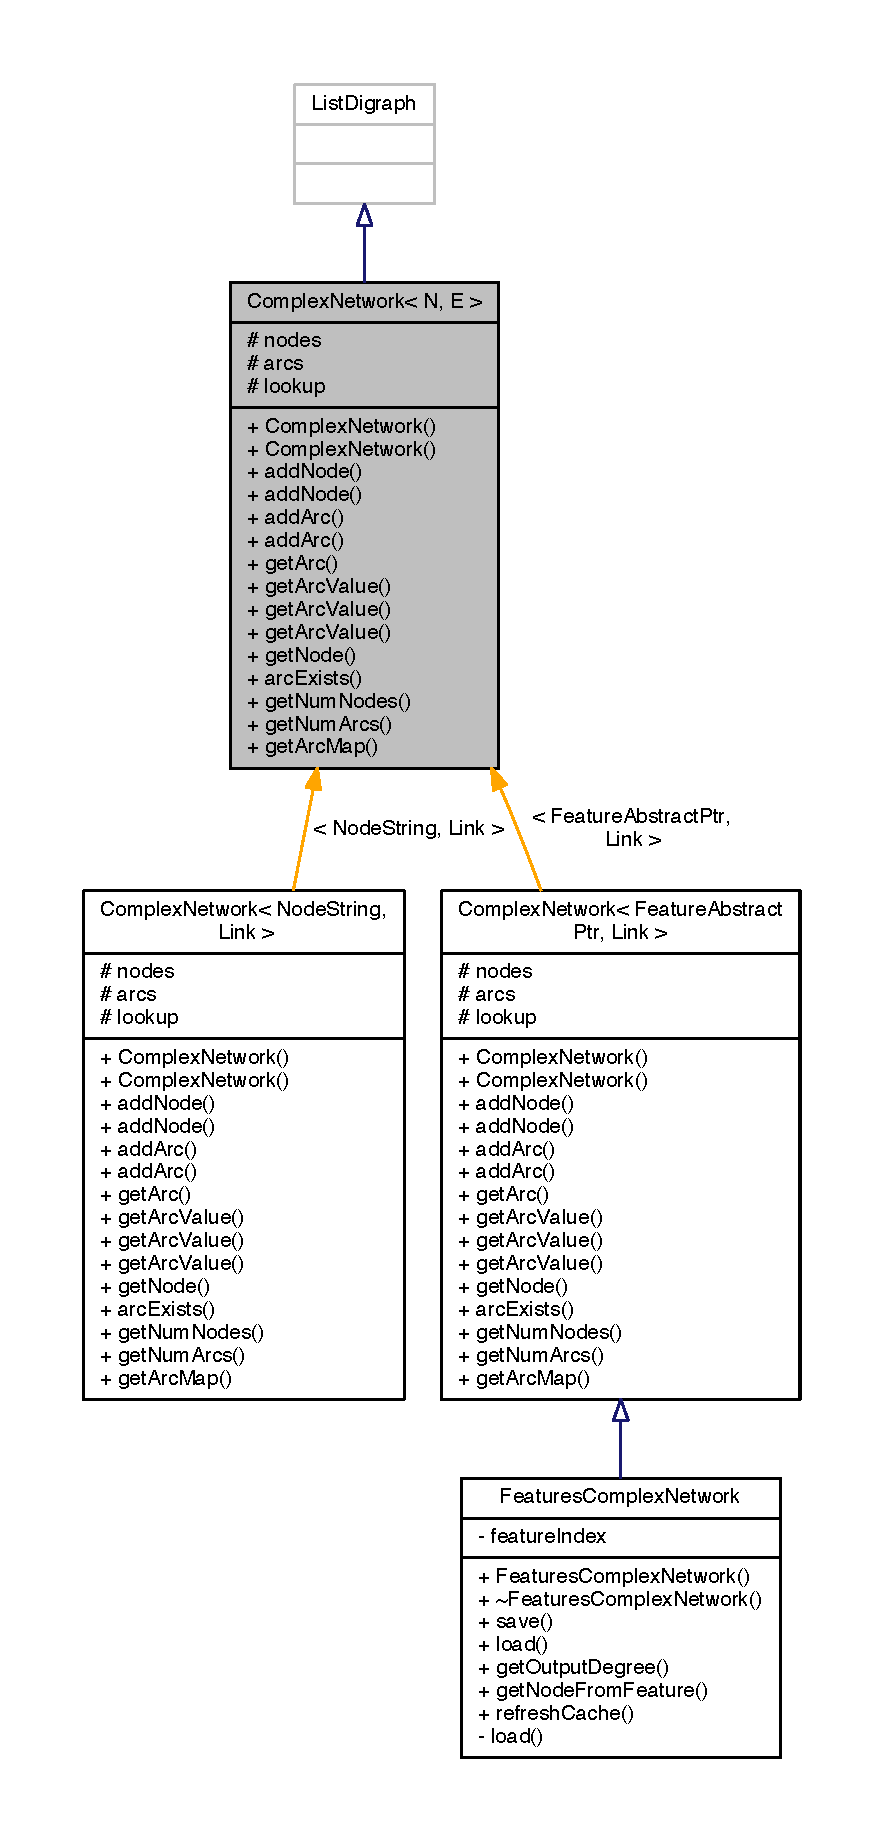
\includegraphics[width=254pt]{class_complex_network__inherit__graph}
\end{center}
\end{figure}


Collaboration diagram for Complex\+Network$<$ N\+O\+D\+E\+\_\+\+T\+Y\+P\+E, E\+D\+G\+E\+\_\+\+T\+Y\+P\+E $>$\+:\nopagebreak
\begin{figure}[H]
\begin{center}
\leavevmode
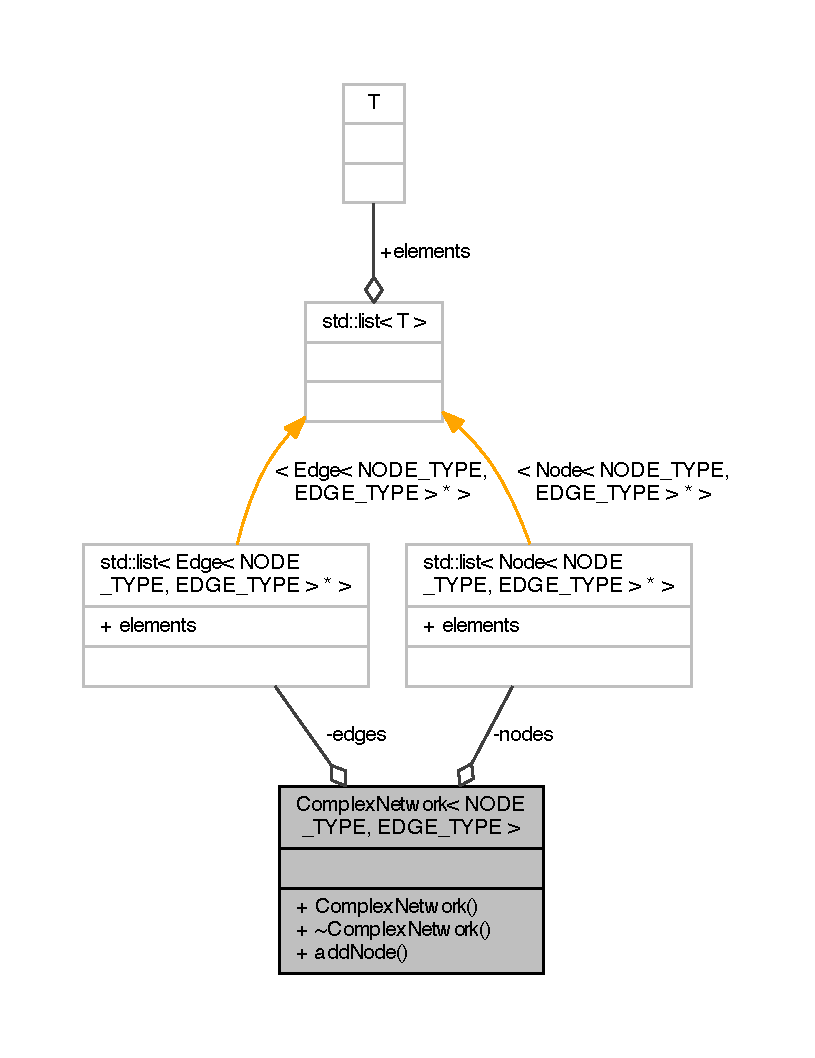
\includegraphics[width=350pt]{class_complex_network__coll__graph}
\end{center}
\end{figure}


\subsection{Constructor \& Destructor Documentation}
\hypertarget{class_complex_network_a4a16e825e1d8b487067ca21d677617a3}{\index{Complex\+Network@{Complex\+Network}!Complex\+Network@{Complex\+Network}}
\index{Complex\+Network@{Complex\+Network}!Complex\+Network@{Complex\+Network}}
\subsubsection[{Complex\+Network}]{\setlength{\rightskip}{0pt plus 5cm}template$<$typename N\+O\+D\+E\+\_\+\+T\+Y\+P\+E , typename E\+D\+G\+E\+\_\+\+T\+Y\+P\+E $>$ {\bf Complex\+Network}$<$ N\+O\+D\+E\+\_\+\+T\+Y\+P\+E, E\+D\+G\+E\+\_\+\+T\+Y\+P\+E $>$\+::{\bf Complex\+Network} (
\begin{DoxyParamCaption}
\item[{bool}]{directed = {\ttfamily true}}
\end{DoxyParamCaption}
)}}\label{class_complex_network_a4a16e825e1d8b487067ca21d677617a3}


\subsection{Member Function Documentation}
\hypertarget{class_complex_network_a52c25eb9c9c642a39681e4040fc0a17d}{\index{Complex\+Network@{Complex\+Network}!add\+Edge@{add\+Edge}}
\index{add\+Edge@{add\+Edge}!Complex\+Network@{Complex\+Network}}
\subsubsection[{add\+Edge}]{\setlength{\rightskip}{0pt plus 5cm}template$<$typename N\+O\+D\+E\+\_\+\+T\+Y\+P\+E , typename E\+D\+G\+E\+\_\+\+T\+Y\+P\+E$>$ void {\bf Complex\+Network}$<$ N\+O\+D\+E\+\_\+\+T\+Y\+P\+E, E\+D\+G\+E\+\_\+\+T\+Y\+P\+E $>$\+::add\+Edge (
\begin{DoxyParamCaption}
\item[{{\bf node\+\_\+id}}]{from, }
\item[{{\bf node\+\_\+id}}]{to, }
\item[{const E\+D\+G\+E\+\_\+\+T\+Y\+P\+E \&}]{e}
\end{DoxyParamCaption}
)\hspace{0.3cm}{\ttfamily [virtual]}}}\label{class_complex_network_a52c25eb9c9c642a39681e4040fc0a17d}


Here is the caller graph for this function\+:
\nopagebreak
\begin{figure}[H]
\begin{center}
\leavevmode
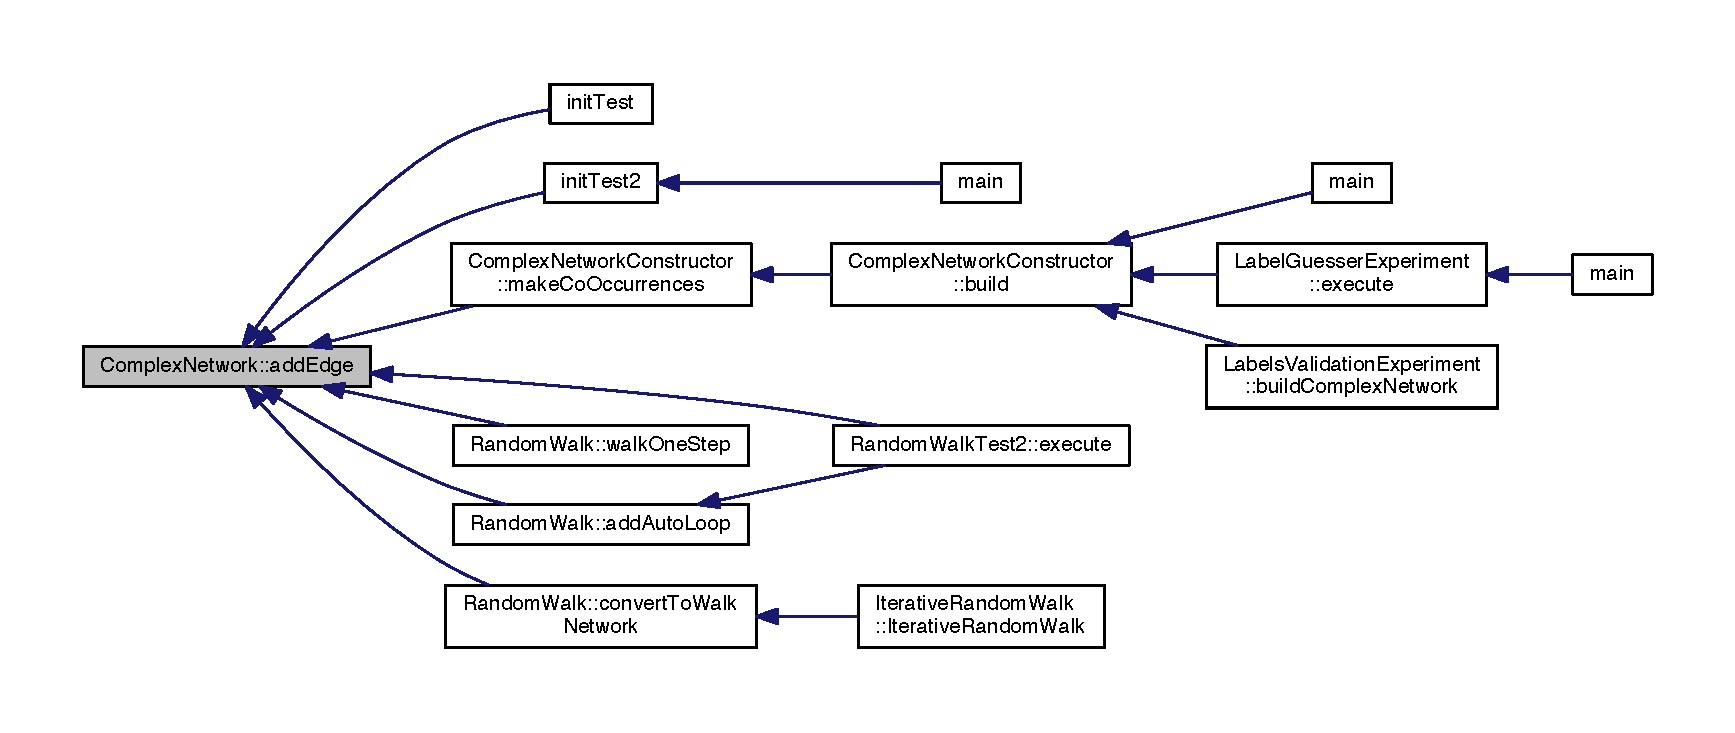
\includegraphics[width=350pt]{class_complex_network_a52c25eb9c9c642a39681e4040fc0a17d_icgraph}
\end{center}
\end{figure}


\hypertarget{class_complex_network_af2c31ca0d2142dafa1d88ca3ff22356f}{\index{Complex\+Network@{Complex\+Network}!add\+Node@{add\+Node}}
\index{add\+Node@{add\+Node}!Complex\+Network@{Complex\+Network}}
\subsubsection[{add\+Node}]{\setlength{\rightskip}{0pt plus 5cm}template$<$typename N\+O\+D\+E\+\_\+\+T\+Y\+P\+E, typename E\+D\+G\+E\+\_\+\+T\+Y\+P\+E $>$ {\bf node\+\_\+id} {\bf Complex\+Network}$<$ N\+O\+D\+E\+\_\+\+T\+Y\+P\+E, E\+D\+G\+E\+\_\+\+T\+Y\+P\+E $>$\+::add\+Node (
\begin{DoxyParamCaption}
\item[{const N\+O\+D\+E\+\_\+\+T\+Y\+P\+E \&}]{n}
\end{DoxyParamCaption}
)\hspace{0.3cm}{\ttfamily [virtual]}}}\label{class_complex_network_af2c31ca0d2142dafa1d88ca3ff22356f}


Reimplemented in \hyperlink{class_cached_complex_network_ad6e24699a050f5f2d7f908aba40b931c}{Cached\+Complex\+Network$<$ N\+O\+D\+E\+\_\+\+T\+Y\+P\+E, E\+D\+G\+E\+\_\+\+T\+Y\+P\+E $>$}, and \hyperlink{class_cached_complex_network_ad6e24699a050f5f2d7f908aba40b931c}{Cached\+Complex\+Network$<$ int, double $>$}.



Here is the caller graph for this function\+:
\nopagebreak
\begin{figure}[H]
\begin{center}
\leavevmode
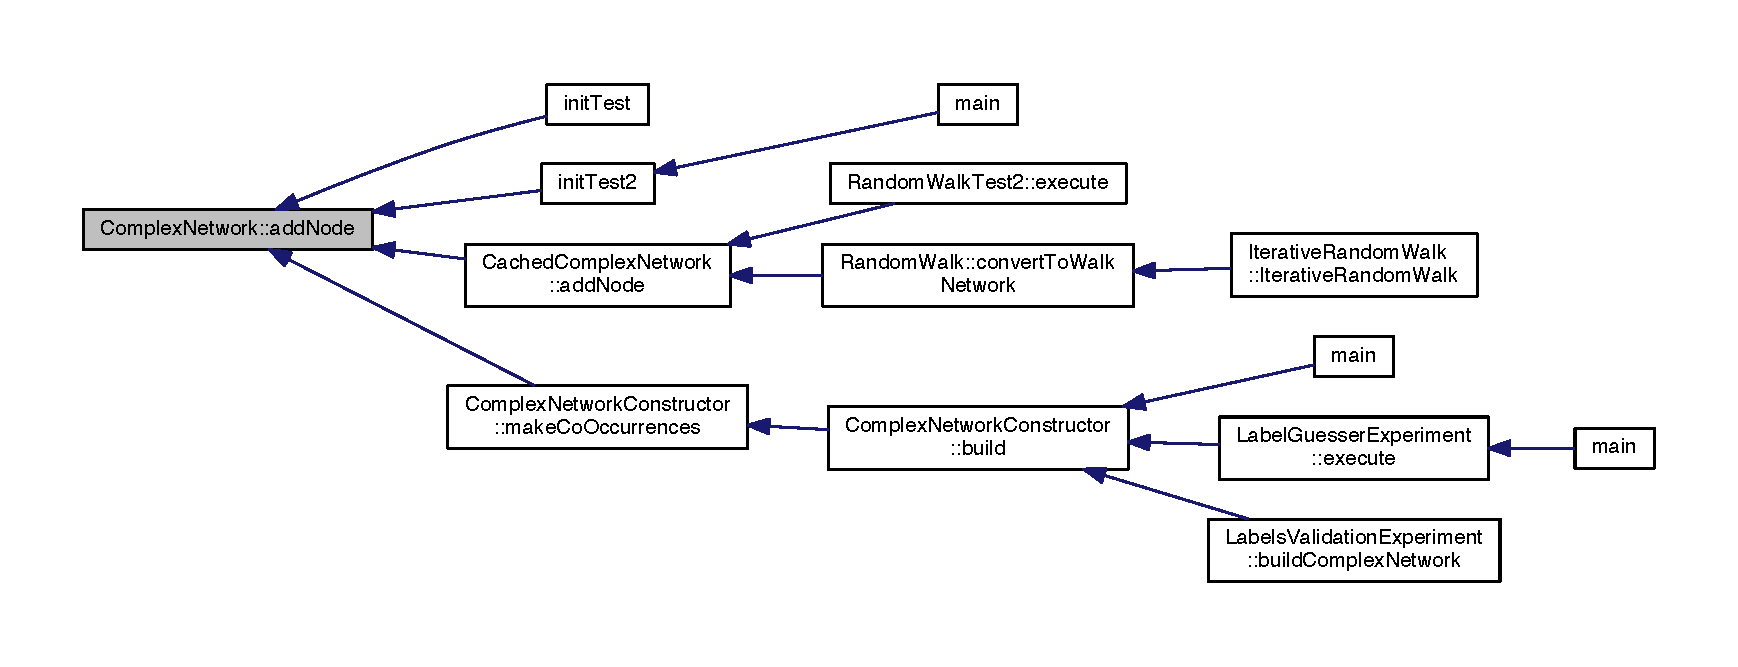
\includegraphics[width=350pt]{class_complex_network_af2c31ca0d2142dafa1d88ca3ff22356f_icgraph}
\end{center}
\end{figure}


\hypertarget{class_complex_network_ab02bc6912437322f146f6ce98b415759}{\index{Complex\+Network@{Complex\+Network}!Begin@{Begin}}
\index{Begin@{Begin}!Complex\+Network@{Complex\+Network}}
\subsubsection[{Begin}]{\setlength{\rightskip}{0pt plus 5cm}template$<$typename N\+O\+D\+E\+\_\+\+T\+Y\+P\+E , typename E\+D\+G\+E\+\_\+\+T\+Y\+P\+E $>$ {\bf Complex\+Network}$<$ N\+O\+D\+E\+\_\+\+T\+Y\+P\+E, E\+D\+G\+E\+\_\+\+T\+Y\+P\+E $>$\+::{\bf Node\+Iterator} {\bf Complex\+Network}$<$ N\+O\+D\+E\+\_\+\+T\+Y\+P\+E, E\+D\+G\+E\+\_\+\+T\+Y\+P\+E $>$\+::Begin (
\begin{DoxyParamCaption}
{}
\end{DoxyParamCaption}
)}}\label{class_complex_network_ab02bc6912437322f146f6ce98b415759}


Here is the caller graph for this function\+:
\nopagebreak
\begin{figure}[H]
\begin{center}
\leavevmode
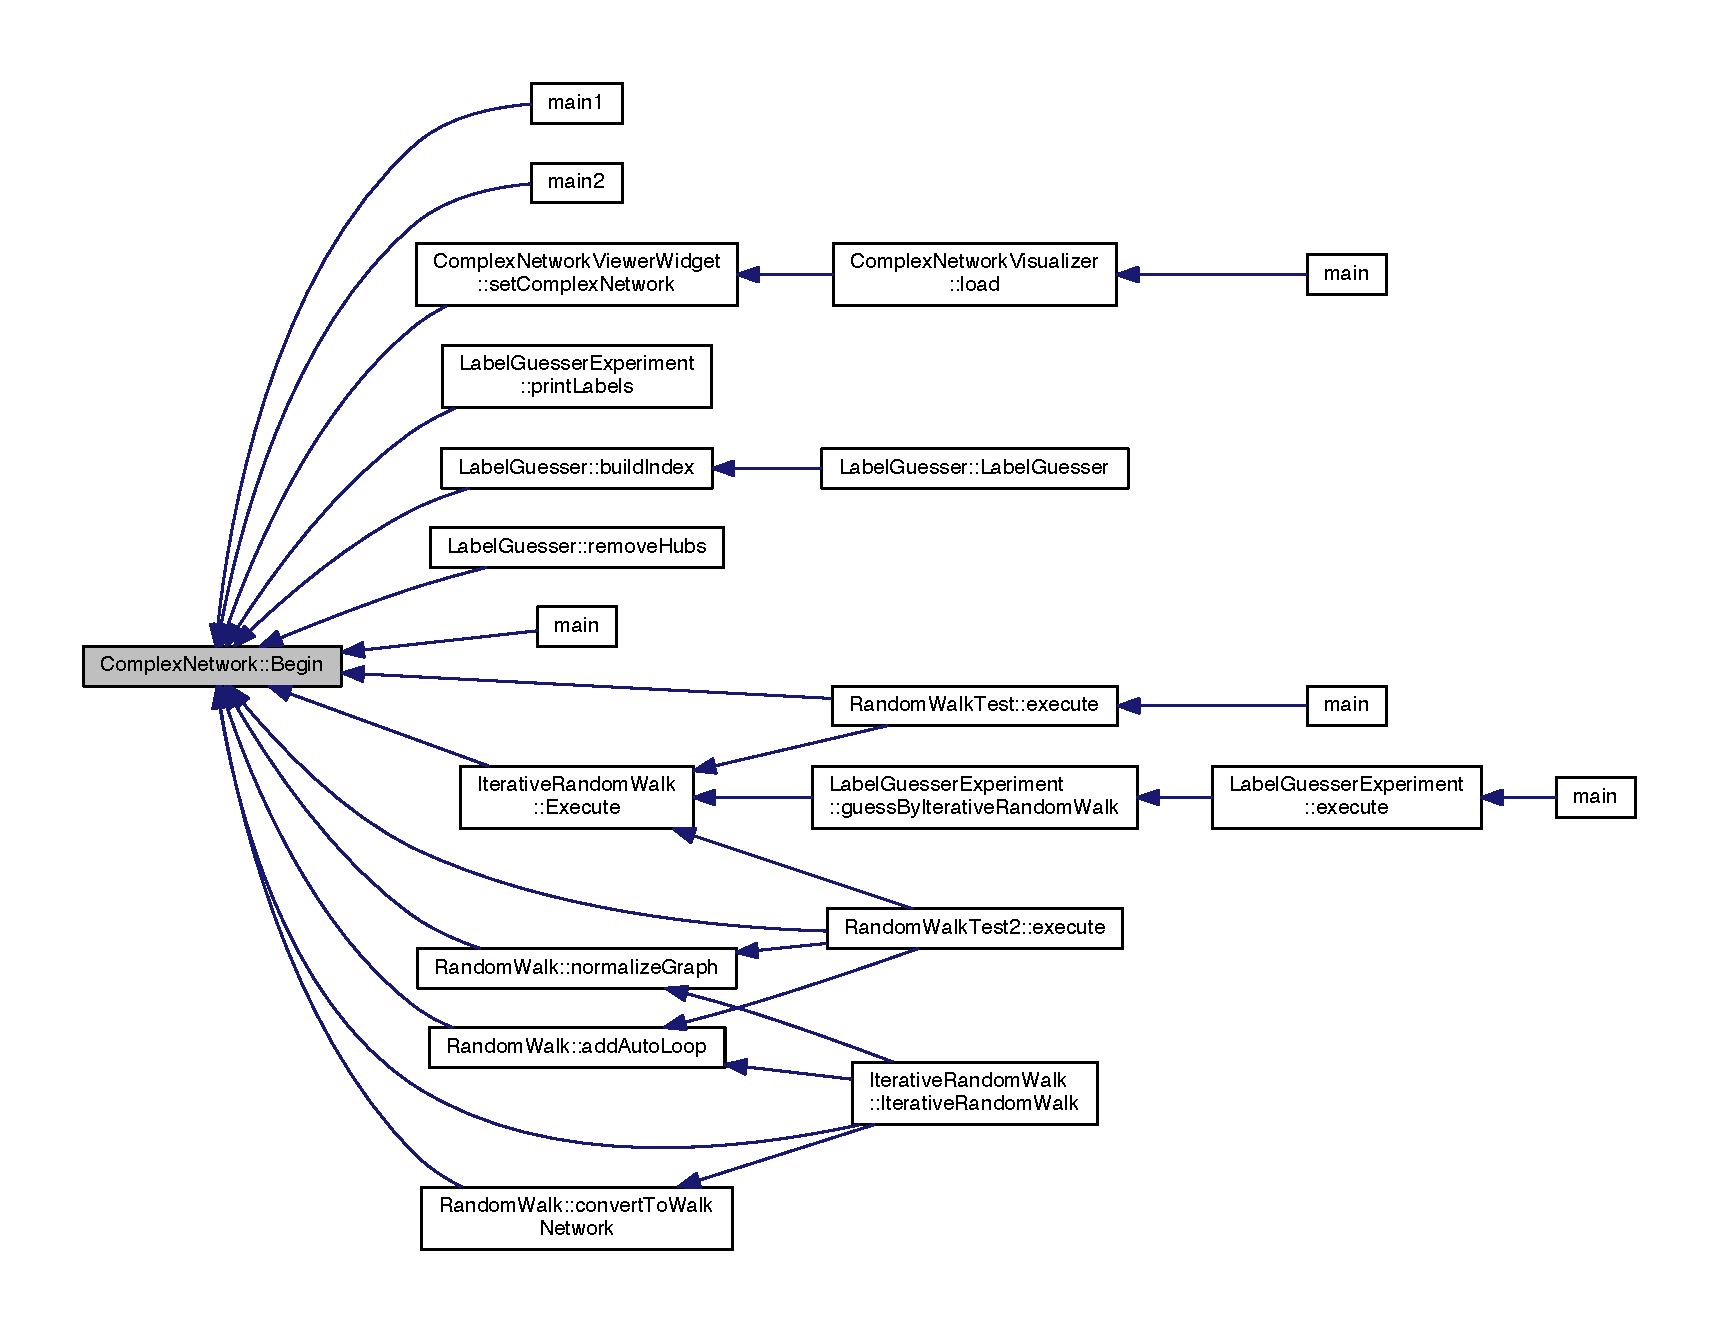
\includegraphics[width=350pt]{class_complex_network_ab02bc6912437322f146f6ce98b415759_icgraph}
\end{center}
\end{figure}


\hypertarget{class_complex_network_a64db5949375a84eba3d9ff559d68fc6e}{\index{Complex\+Network@{Complex\+Network}!clear@{clear}}
\index{clear@{clear}!Complex\+Network@{Complex\+Network}}
\subsubsection[{clear}]{\setlength{\rightskip}{0pt plus 5cm}template$<$typename N\+O\+D\+E\+\_\+\+T\+Y\+P\+E , typename E\+D\+G\+E\+\_\+\+T\+Y\+P\+E $>$ void {\bf Complex\+Network}$<$ N\+O\+D\+E\+\_\+\+T\+Y\+P\+E, E\+D\+G\+E\+\_\+\+T\+Y\+P\+E $>$\+::clear (
\begin{DoxyParamCaption}
{}
\end{DoxyParamCaption}
)\hspace{0.3cm}{\ttfamily [virtual]}}}\label{class_complex_network_a64db5949375a84eba3d9ff559d68fc6e}


Reimplemented in \hyperlink{class_features_complex_network_a747eba83de2a19a39e3d9f230d055d59}{Features\+Complex\+Network}.

\hypertarget{class_complex_network_a982b0db93143ff949025e326794af02d}{\index{Complex\+Network@{Complex\+Network}!create\+Edge\+Key@{create\+Edge\+Key}}
\index{create\+Edge\+Key@{create\+Edge\+Key}!Complex\+Network@{Complex\+Network}}
\subsubsection[{create\+Edge\+Key}]{\setlength{\rightskip}{0pt plus 5cm}template$<$typename N\+O\+D\+E\+\_\+\+T\+Y\+P\+E , typename E\+D\+G\+E\+\_\+\+T\+Y\+P\+E $>$ Q\+Pair$<$ {\bf node\+\_\+id}, {\bf node\+\_\+id} $>$ {\bf Complex\+Network}$<$ N\+O\+D\+E\+\_\+\+T\+Y\+P\+E, E\+D\+G\+E\+\_\+\+T\+Y\+P\+E $>$\+::create\+Edge\+Key (
\begin{DoxyParamCaption}
\item[{{\bf node\+\_\+id}}]{from, }
\item[{{\bf node\+\_\+id}}]{to}
\end{DoxyParamCaption}
)\hspace{0.3cm}{\ttfamily [inline]}, {\ttfamily [protected]}}}\label{class_complex_network_a982b0db93143ff949025e326794af02d}
\hypertarget{class_complex_network_a2167b224079f5c0b44443959ad0b6440}{\index{Complex\+Network@{Complex\+Network}!Edges\+Begin@{Edges\+Begin}}
\index{Edges\+Begin@{Edges\+Begin}!Complex\+Network@{Complex\+Network}}
\subsubsection[{Edges\+Begin}]{\setlength{\rightskip}{0pt plus 5cm}template$<$typename N\+O\+D\+E\+\_\+\+T\+Y\+P\+E , typename E\+D\+G\+E\+\_\+\+T\+Y\+P\+E $>$ {\bf Complex\+Network}$<$ N\+O\+D\+E\+\_\+\+T\+Y\+P\+E, E\+D\+G\+E\+\_\+\+T\+Y\+P\+E $>$\+::{\bf Edge\+Iterator} {\bf Complex\+Network}$<$ N\+O\+D\+E\+\_\+\+T\+Y\+P\+E, E\+D\+G\+E\+\_\+\+T\+Y\+P\+E $>$\+::Edges\+Begin (
\begin{DoxyParamCaption}
\item[{{\bf node\+\_\+id}}]{node\+\_\+from}
\end{DoxyParamCaption}
)}}\label{class_complex_network_a2167b224079f5c0b44443959ad0b6440}


Here is the caller graph for this function\+:\nopagebreak
\begin{figure}[H]
\begin{center}
\leavevmode
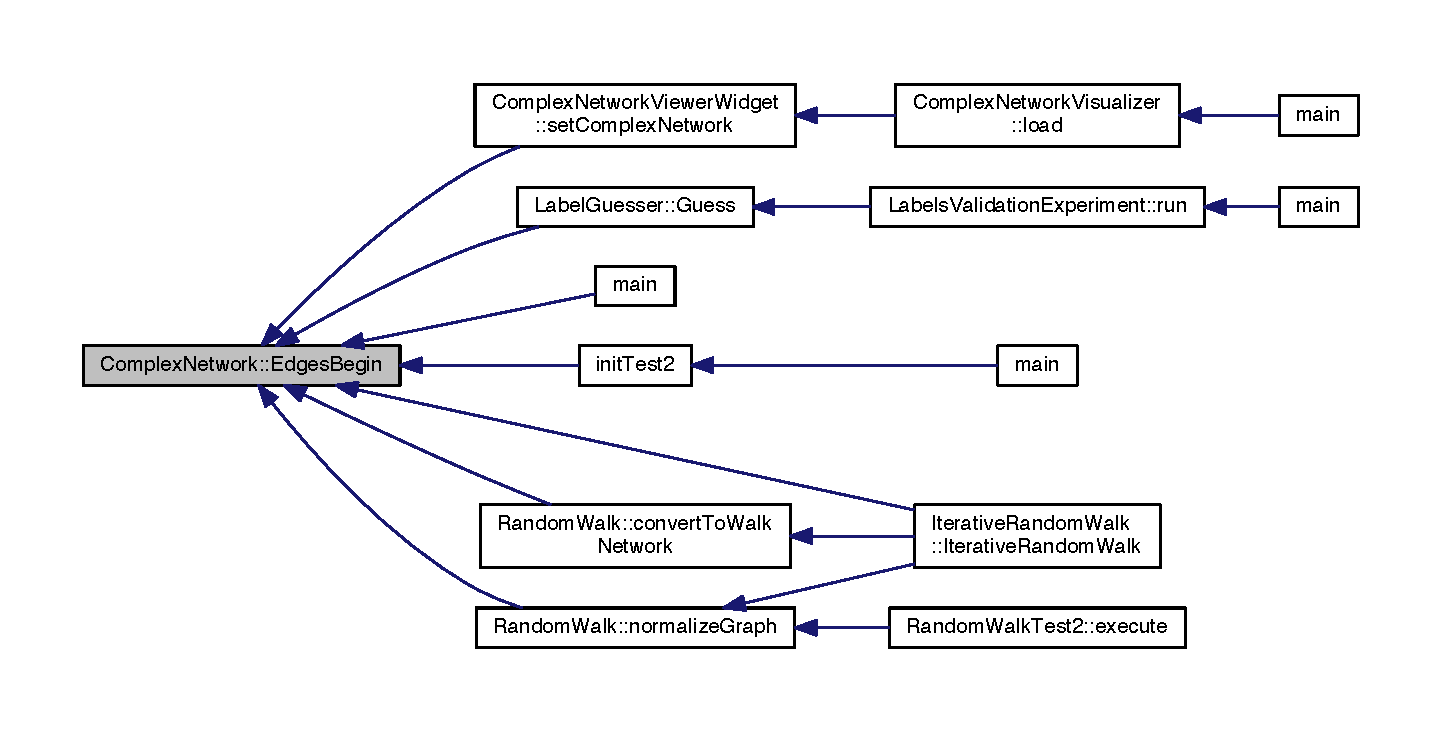
\includegraphics[width=350pt]{class_complex_network_a2167b224079f5c0b44443959ad0b6440_icgraph}
\end{center}
\end{figure}


\hypertarget{class_complex_network_a3a228b9a9497db2b9385deb4eb39f1e1}{\index{Complex\+Network@{Complex\+Network}!Edges\+Begin@{Edges\+Begin}}
\index{Edges\+Begin@{Edges\+Begin}!Complex\+Network@{Complex\+Network}}
\subsubsection[{Edges\+Begin}]{\setlength{\rightskip}{0pt plus 5cm}template$<$typename N\+O\+D\+E\+\_\+\+T\+Y\+P\+E , typename E\+D\+G\+E\+\_\+\+T\+Y\+P\+E $>$ {\bf Complex\+Network}$<$ N\+O\+D\+E\+\_\+\+T\+Y\+P\+E, E\+D\+G\+E\+\_\+\+T\+Y\+P\+E $>$\+::{\bf Edge\+Iterator} {\bf Complex\+Network}$<$ N\+O\+D\+E\+\_\+\+T\+Y\+P\+E, E\+D\+G\+E\+\_\+\+T\+Y\+P\+E $>$\+::Edges\+Begin (
\begin{DoxyParamCaption}
{}
\end{DoxyParamCaption}
)}}\label{class_complex_network_a3a228b9a9497db2b9385deb4eb39f1e1}
\hypertarget{class_complex_network_ad806138ea94ec18ed17f4681ab731208}{\index{Complex\+Network@{Complex\+Network}!Edges\+End@{Edges\+End}}
\index{Edges\+End@{Edges\+End}!Complex\+Network@{Complex\+Network}}
\subsubsection[{Edges\+End}]{\setlength{\rightskip}{0pt plus 5cm}template$<$typename N\+O\+D\+E\+\_\+\+T\+Y\+P\+E , typename E\+D\+G\+E\+\_\+\+T\+Y\+P\+E $>$ {\bf Complex\+Network}$<$ N\+O\+D\+E\+\_\+\+T\+Y\+P\+E, E\+D\+G\+E\+\_\+\+T\+Y\+P\+E $>$\+::{\bf Edge\+Iterator} {\bf Complex\+Network}$<$ N\+O\+D\+E\+\_\+\+T\+Y\+P\+E, E\+D\+G\+E\+\_\+\+T\+Y\+P\+E $>$\+::Edges\+End (
\begin{DoxyParamCaption}
\item[{{\bf node\+\_\+id}}]{node\+\_\+from}
\end{DoxyParamCaption}
)}}\label{class_complex_network_ad806138ea94ec18ed17f4681ab731208}


Here is the caller graph for this function\+:\nopagebreak
\begin{figure}[H]
\begin{center}
\leavevmode
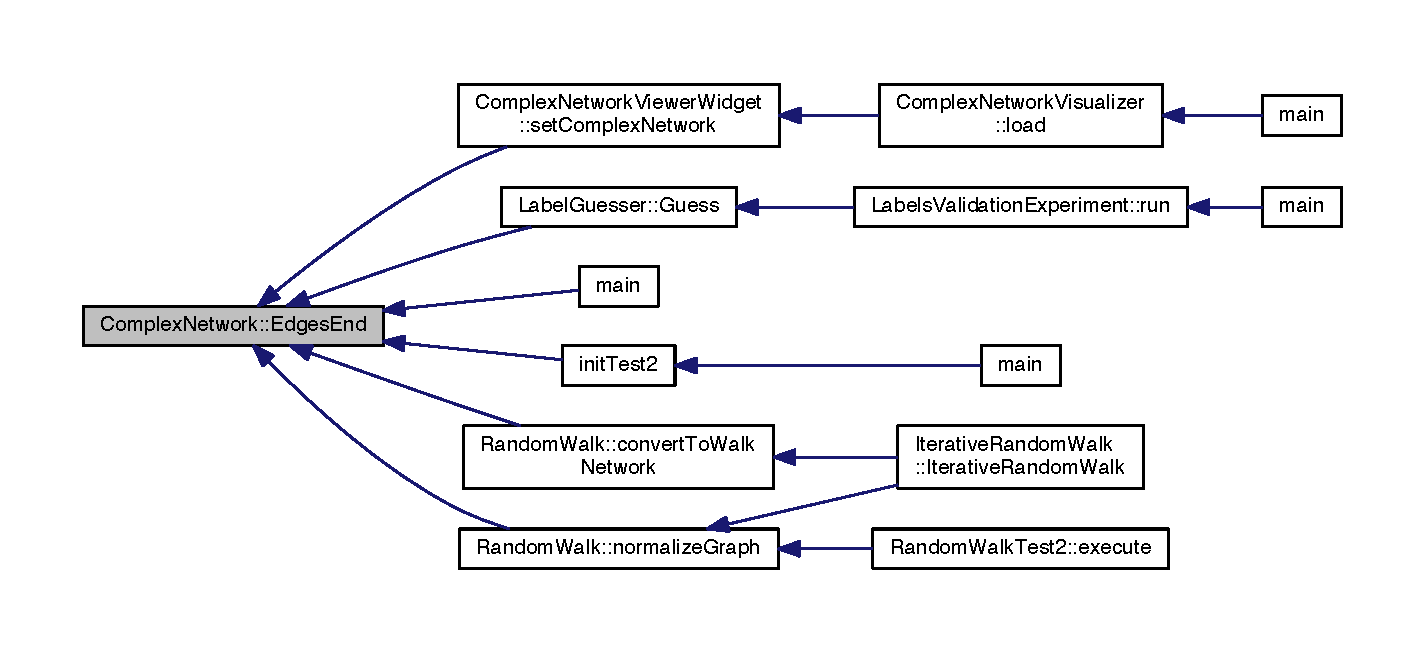
\includegraphics[width=350pt]{class_complex_network_ad806138ea94ec18ed17f4681ab731208_icgraph}
\end{center}
\end{figure}


\hypertarget{class_complex_network_afa7d628b66a815d97afbf5373640d12b}{\index{Complex\+Network@{Complex\+Network}!Edges\+End@{Edges\+End}}
\index{Edges\+End@{Edges\+End}!Complex\+Network@{Complex\+Network}}
\subsubsection[{Edges\+End}]{\setlength{\rightskip}{0pt plus 5cm}template$<$typename N\+O\+D\+E\+\_\+\+T\+Y\+P\+E , typename E\+D\+G\+E\+\_\+\+T\+Y\+P\+E $>$ {\bf Complex\+Network}$<$ N\+O\+D\+E\+\_\+\+T\+Y\+P\+E, E\+D\+G\+E\+\_\+\+T\+Y\+P\+E $>$\+::{\bf Edge\+Iterator} {\bf Complex\+Network}$<$ N\+O\+D\+E\+\_\+\+T\+Y\+P\+E, E\+D\+G\+E\+\_\+\+T\+Y\+P\+E $>$\+::Edges\+End (
\begin{DoxyParamCaption}
{}
\end{DoxyParamCaption}
)}}\label{class_complex_network_afa7d628b66a815d97afbf5373640d12b}
\hypertarget{class_complex_network_a2c90f4efd046776d7a53776b24daae0f}{\index{Complex\+Network@{Complex\+Network}!End@{End}}
\index{End@{End}!Complex\+Network@{Complex\+Network}}
\subsubsection[{End}]{\setlength{\rightskip}{0pt plus 5cm}template$<$typename N\+O\+D\+E\+\_\+\+T\+Y\+P\+E , typename E\+D\+G\+E\+\_\+\+T\+Y\+P\+E $>$ {\bf Complex\+Network}$<$ N\+O\+D\+E\+\_\+\+T\+Y\+P\+E, E\+D\+G\+E\+\_\+\+T\+Y\+P\+E $>$\+::{\bf Node\+Iterator} {\bf Complex\+Network}$<$ N\+O\+D\+E\+\_\+\+T\+Y\+P\+E, E\+D\+G\+E\+\_\+\+T\+Y\+P\+E $>$\+::End (
\begin{DoxyParamCaption}
{}
\end{DoxyParamCaption}
)}}\label{class_complex_network_a2c90f4efd046776d7a53776b24daae0f}


Here is the caller graph for this function\+:
\nopagebreak
\begin{figure}[H]
\begin{center}
\leavevmode
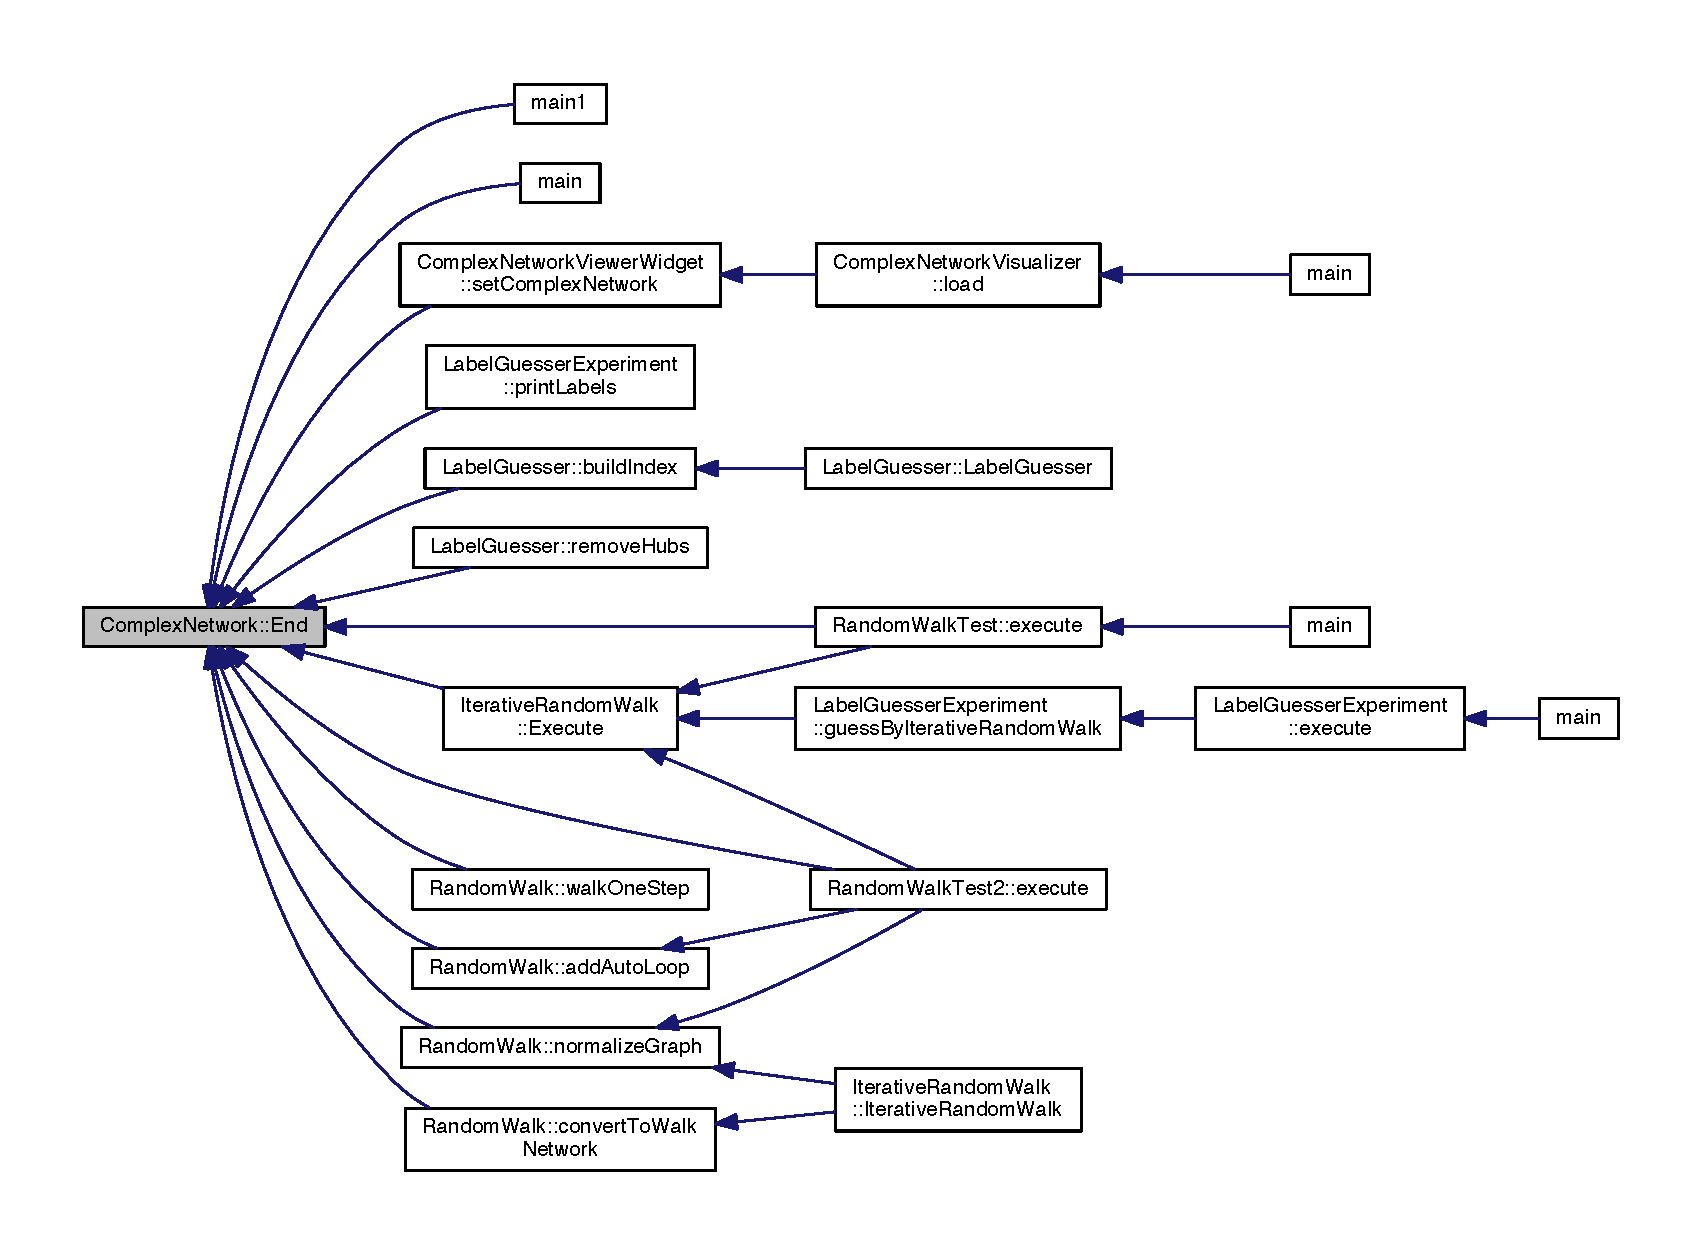
\includegraphics[width=350pt]{class_complex_network_a2c90f4efd046776d7a53776b24daae0f_icgraph}
\end{center}
\end{figure}


\hypertarget{class_complex_network_a6a1c638e4604efe06c12ce3065020ec1}{\index{Complex\+Network@{Complex\+Network}!get\+Edge@{get\+Edge}}
\index{get\+Edge@{get\+Edge}!Complex\+Network@{Complex\+Network}}
\subsubsection[{get\+Edge}]{\setlength{\rightskip}{0pt plus 5cm}template$<$typename N\+O\+D\+E\+\_\+\+T\+Y\+P\+E , typename E\+D\+G\+E\+\_\+\+T\+Y\+P\+E $>$ E\+D\+G\+E\+\_\+\+T\+Y\+P\+E $\ast$ {\bf Complex\+Network}$<$ N\+O\+D\+E\+\_\+\+T\+Y\+P\+E, E\+D\+G\+E\+\_\+\+T\+Y\+P\+E $>$\+::get\+Edge (
\begin{DoxyParamCaption}
\item[{{\bf node\+\_\+id}}]{from, }
\item[{{\bf node\+\_\+id}}]{to}
\end{DoxyParamCaption}
)\hspace{0.3cm}{\ttfamily [virtual]}}}\label{class_complex_network_a6a1c638e4604efe06c12ce3065020ec1}


Here is the caller graph for this function\+:
\nopagebreak
\begin{figure}[H]
\begin{center}
\leavevmode
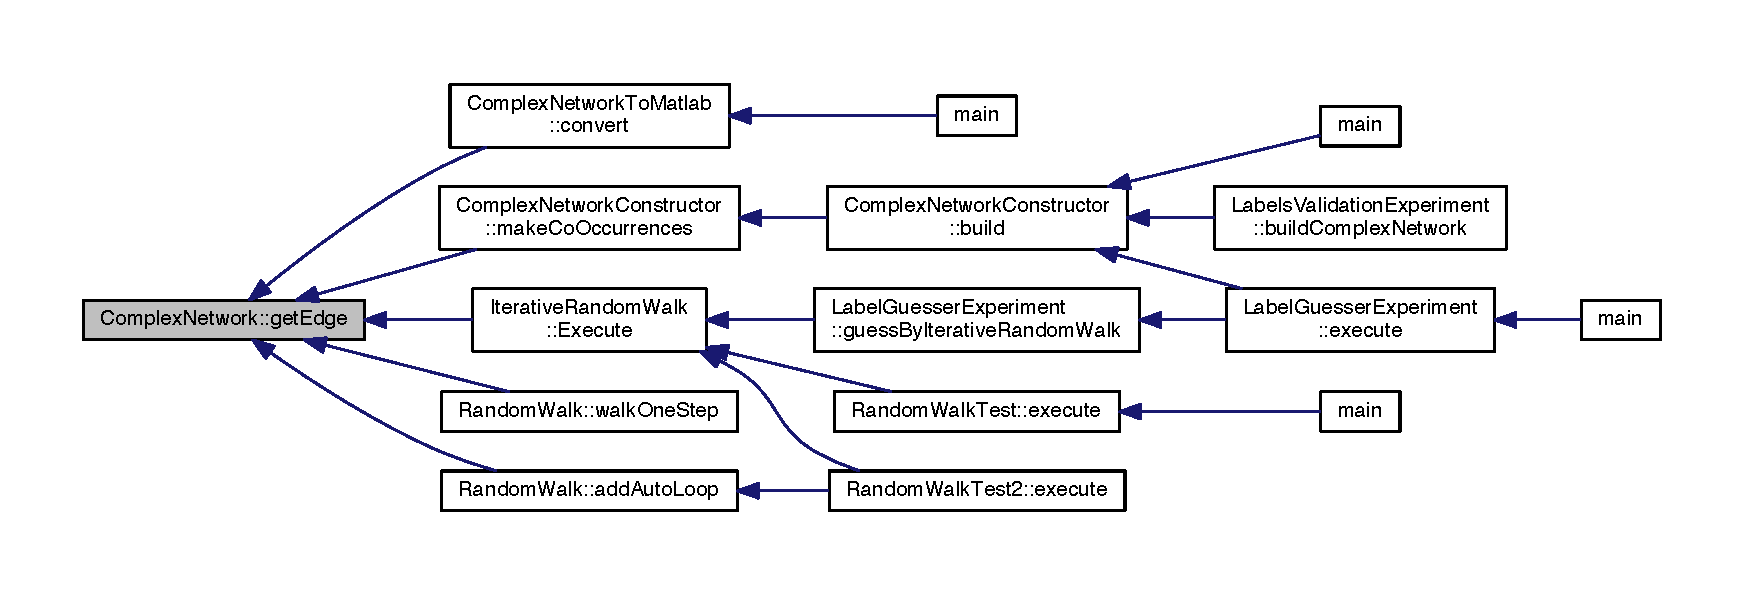
\includegraphics[width=350pt]{class_complex_network_a6a1c638e4604efe06c12ce3065020ec1_icgraph}
\end{center}
\end{figure}


\hypertarget{class_complex_network_ad440008416fc33500754d77b2532560f}{\index{Complex\+Network@{Complex\+Network}!get\+Edge\+From\+Edge\+Id@{get\+Edge\+From\+Edge\+Id}}
\index{get\+Edge\+From\+Edge\+Id@{get\+Edge\+From\+Edge\+Id}!Complex\+Network@{Complex\+Network}}
\subsubsection[{get\+Edge\+From\+Edge\+Id}]{\setlength{\rightskip}{0pt plus 5cm}template$<$typename N\+O\+D\+E\+\_\+\+T\+Y\+P\+E , typename E\+D\+G\+E\+\_\+\+T\+Y\+P\+E $>$ E\+D\+G\+E\+\_\+\+T\+Y\+P\+E $\ast$ {\bf Complex\+Network}$<$ N\+O\+D\+E\+\_\+\+T\+Y\+P\+E, E\+D\+G\+E\+\_\+\+T\+Y\+P\+E $>$\+::get\+Edge\+From\+Edge\+Id (
\begin{DoxyParamCaption}
\item[{{\bf edge\+\_\+id}}]{id}
\end{DoxyParamCaption}
)\hspace{0.3cm}{\ttfamily [virtual]}}}\label{class_complex_network_ad440008416fc33500754d77b2532560f}
\hypertarget{class_complex_network_a3711aff250a942a9ad61d0571be82c43}{\index{Complex\+Network@{Complex\+Network}!get\+Node@{get\+Node}}
\index{get\+Node@{get\+Node}!Complex\+Network@{Complex\+Network}}
\subsubsection[{get\+Node}]{\setlength{\rightskip}{0pt plus 5cm}template$<$typename N\+O\+D\+E\+\_\+\+T\+Y\+P\+E , typename E\+D\+G\+E\+\_\+\+T\+Y\+P\+E $>$ N\+O\+D\+E\+\_\+\+T\+Y\+P\+E $\ast$ {\bf Complex\+Network}$<$ N\+O\+D\+E\+\_\+\+T\+Y\+P\+E, E\+D\+G\+E\+\_\+\+T\+Y\+P\+E $>$\+::get\+Node (
\begin{DoxyParamCaption}
\item[{{\bf node\+\_\+id}}]{id}
\end{DoxyParamCaption}
)\hspace{0.3cm}{\ttfamily [virtual]}}}\label{class_complex_network_a3711aff250a942a9ad61d0571be82c43}


Here is the caller graph for this function\+:
\nopagebreak
\begin{figure}[H]
\begin{center}
\leavevmode
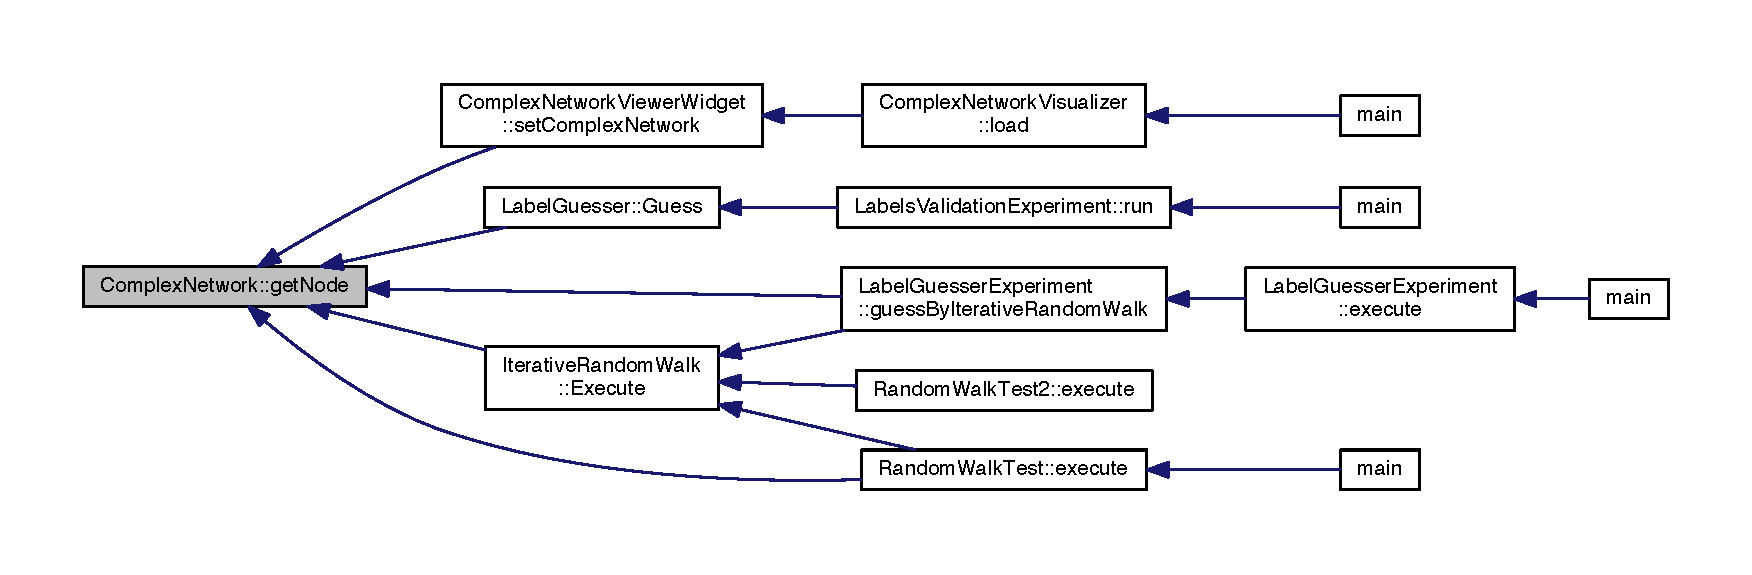
\includegraphics[width=350pt]{class_complex_network_a3711aff250a942a9ad61d0571be82c43_icgraph}
\end{center}
\end{figure}


\hypertarget{class_complex_network_a720cb4e40342648d394792cc693d29a5}{\index{Complex\+Network@{Complex\+Network}!get\+Num\+Edges@{get\+Num\+Edges}}
\index{get\+Num\+Edges@{get\+Num\+Edges}!Complex\+Network@{Complex\+Network}}
\subsubsection[{get\+Num\+Edges}]{\setlength{\rightskip}{0pt plus 5cm}template$<$typename N\+O\+D\+E\+\_\+\+T\+Y\+P\+E , typename E\+D\+G\+E\+\_\+\+T\+Y\+P\+E $>$ unsigned int {\bf Complex\+Network}$<$ N\+O\+D\+E\+\_\+\+T\+Y\+P\+E, E\+D\+G\+E\+\_\+\+T\+Y\+P\+E $>$\+::get\+Num\+Edges (
\begin{DoxyParamCaption}
{}
\end{DoxyParamCaption}
) const}}\label{class_complex_network_a720cb4e40342648d394792cc693d29a5}


Here is the caller graph for this function\+:\nopagebreak
\begin{figure}[H]
\begin{center}
\leavevmode
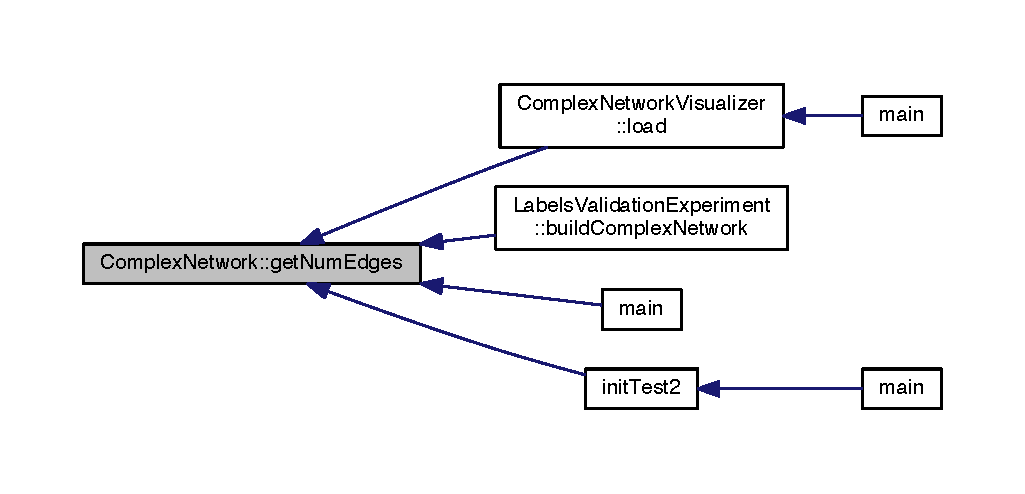
\includegraphics[width=350pt]{class_complex_network_a720cb4e40342648d394792cc693d29a5_icgraph}
\end{center}
\end{figure}


\hypertarget{class_complex_network_a4036d2cda2dc5596d03e164c3455aff6}{\index{Complex\+Network@{Complex\+Network}!get\+Num\+Edges@{get\+Num\+Edges}}
\index{get\+Num\+Edges@{get\+Num\+Edges}!Complex\+Network@{Complex\+Network}}
\subsubsection[{get\+Num\+Edges}]{\setlength{\rightskip}{0pt plus 5cm}template$<$typename N\+O\+D\+E\+\_\+\+T\+Y\+P\+E , typename E\+D\+G\+E\+\_\+\+T\+Y\+P\+E $>$ unsigned int {\bf Complex\+Network}$<$ N\+O\+D\+E\+\_\+\+T\+Y\+P\+E, E\+D\+G\+E\+\_\+\+T\+Y\+P\+E $>$\+::get\+Num\+Edges (
\begin{DoxyParamCaption}
\item[{{\bf node\+\_\+id}}]{id}
\end{DoxyParamCaption}
) const}}\label{class_complex_network_a4036d2cda2dc5596d03e164c3455aff6}
\hypertarget{class_complex_network_afee98f26ceed674c17be01a740787170}{\index{Complex\+Network@{Complex\+Network}!get\+Num\+Nodes@{get\+Num\+Nodes}}
\index{get\+Num\+Nodes@{get\+Num\+Nodes}!Complex\+Network@{Complex\+Network}}
\subsubsection[{get\+Num\+Nodes}]{\setlength{\rightskip}{0pt plus 5cm}template$<$typename N\+O\+D\+E\+\_\+\+T\+Y\+P\+E , typename E\+D\+G\+E\+\_\+\+T\+Y\+P\+E $>$ unsigned int {\bf Complex\+Network}$<$ N\+O\+D\+E\+\_\+\+T\+Y\+P\+E, E\+D\+G\+E\+\_\+\+T\+Y\+P\+E $>$\+::get\+Num\+Nodes (
\begin{DoxyParamCaption}
{}
\end{DoxyParamCaption}
) const}}\label{class_complex_network_afee98f26ceed674c17be01a740787170}


Here is the caller graph for this function\+:
\nopagebreak
\begin{figure}[H]
\begin{center}
\leavevmode
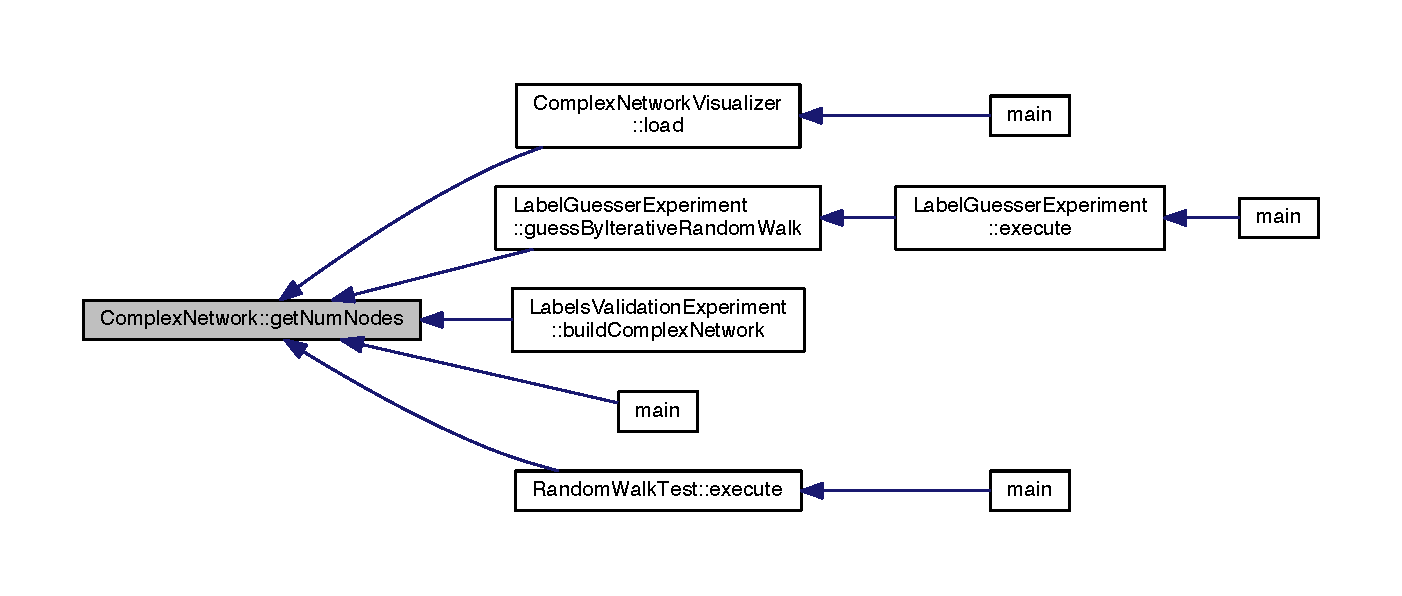
\includegraphics[width=350pt]{class_complex_network_afee98f26ceed674c17be01a740787170_icgraph}
\end{center}
\end{figure}


\hypertarget{class_complex_network_a54fbdb35418f424e8dad0dbc5dc16bee}{\index{Complex\+Network@{Complex\+Network}!load@{load}}
\index{load@{load}!Complex\+Network@{Complex\+Network}}
\subsubsection[{load}]{\setlength{\rightskip}{0pt plus 5cm}template$<$typename N\+O\+D\+E\+\_\+\+T\+Y\+P\+E , typename E\+D\+G\+E\+\_\+\+T\+Y\+P\+E $>$ void {\bf Complex\+Network}$<$ N\+O\+D\+E\+\_\+\+T\+Y\+P\+E, E\+D\+G\+E\+\_\+\+T\+Y\+P\+E $>$\+::load (
\begin{DoxyParamCaption}
\item[{const char $\ast$}]{filename}
\end{DoxyParamCaption}
)}}\label{class_complex_network_a54fbdb35418f424e8dad0dbc5dc16bee}


Here is the caller graph for this function\+:\nopagebreak
\begin{figure}[H]
\begin{center}
\leavevmode
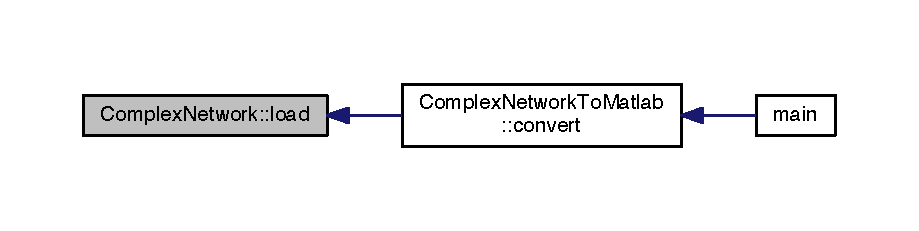
\includegraphics[width=350pt]{class_complex_network_a54fbdb35418f424e8dad0dbc5dc16bee_icgraph}
\end{center}
\end{figure}


\hypertarget{class_complex_network_a5a8b07f5ca5d247e13a2e2bc5ac75de1}{\index{Complex\+Network@{Complex\+Network}!operator=@{operator=}}
\index{operator=@{operator=}!Complex\+Network@{Complex\+Network}}
\subsubsection[{operator=}]{\setlength{\rightskip}{0pt plus 5cm}template$<$typename N\+O\+D\+E\+\_\+\+T\+Y\+P\+E, typename E\+D\+G\+E\+\_\+\+T\+Y\+P\+E$>$ {\bf Complex\+Network}$<$ N\+O\+D\+E\+\_\+\+T\+Y\+P\+E, E\+D\+G\+E\+\_\+\+T\+Y\+P\+E $>$ \& {\bf Complex\+Network}$<$ N\+O\+D\+E\+\_\+\+T\+Y\+P\+E, E\+D\+G\+E\+\_\+\+T\+Y\+P\+E $>$\+::operator= (
\begin{DoxyParamCaption}
\item[{const {\bf Complex\+Network}$<$ N\+O\+D\+E\+\_\+\+T\+Y\+P\+E, E\+D\+G\+E\+\_\+\+T\+Y\+P\+E $>$ \&}]{cn}
\end{DoxyParamCaption}
)}}\label{class_complex_network_a5a8b07f5ca5d247e13a2e2bc5ac75de1}
\hypertarget{class_complex_network_a9b2c7df561a2ad5fc14b04a5c5c56828}{\index{Complex\+Network@{Complex\+Network}!remove\+Edge@{remove\+Edge}}
\index{remove\+Edge@{remove\+Edge}!Complex\+Network@{Complex\+Network}}
\subsubsection[{remove\+Edge}]{\setlength{\rightskip}{0pt plus 5cm}template$<$typename N\+O\+D\+E\+\_\+\+T\+Y\+P\+E , typename E\+D\+G\+E\+\_\+\+T\+Y\+P\+E $>$ bool {\bf Complex\+Network}$<$ N\+O\+D\+E\+\_\+\+T\+Y\+P\+E, E\+D\+G\+E\+\_\+\+T\+Y\+P\+E $>$\+::remove\+Edge (
\begin{DoxyParamCaption}
\item[{{\bf node\+\_\+id}}]{from, }
\item[{{\bf node\+\_\+id}}]{to}
\end{DoxyParamCaption}
)\hspace{0.3cm}{\ttfamily [virtual]}}}\label{class_complex_network_a9b2c7df561a2ad5fc14b04a5c5c56828}


Here is the caller graph for this function\+:\nopagebreak
\begin{figure}[H]
\begin{center}
\leavevmode
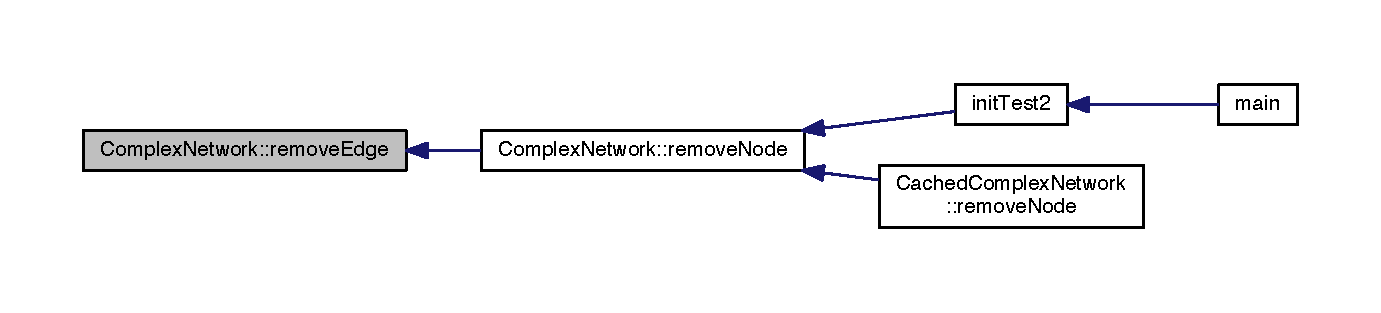
\includegraphics[width=350pt]{class_complex_network_a9b2c7df561a2ad5fc14b04a5c5c56828_icgraph}
\end{center}
\end{figure}


\hypertarget{class_complex_network_a33f2b4528cc31296ede98be7e6dcd600}{\index{Complex\+Network@{Complex\+Network}!remove\+Node@{remove\+Node}}
\index{remove\+Node@{remove\+Node}!Complex\+Network@{Complex\+Network}}
\subsubsection[{remove\+Node}]{\setlength{\rightskip}{0pt plus 5cm}template$<$typename N\+O\+D\+E\+\_\+\+T\+Y\+P\+E , typename E\+D\+G\+E\+\_\+\+T\+Y\+P\+E $>$ bool {\bf Complex\+Network}$<$ N\+O\+D\+E\+\_\+\+T\+Y\+P\+E, E\+D\+G\+E\+\_\+\+T\+Y\+P\+E $>$\+::remove\+Node (
\begin{DoxyParamCaption}
\item[{{\bf node\+\_\+id}}]{id}
\end{DoxyParamCaption}
)\hspace{0.3cm}{\ttfamily [virtual]}}}\label{class_complex_network_a33f2b4528cc31296ede98be7e6dcd600}


Reimplemented in \hyperlink{class_cached_complex_network_a800aa02b94aa4bb73227e139cb246ddf}{Cached\+Complex\+Network$<$ N\+O\+D\+E\+\_\+\+T\+Y\+P\+E, E\+D\+G\+E\+\_\+\+T\+Y\+P\+E $>$}, and \hyperlink{class_cached_complex_network_a800aa02b94aa4bb73227e139cb246ddf}{Cached\+Complex\+Network$<$ int, double $>$}.



Here is the call graph for this function\+:\nopagebreak
\begin{figure}[H]
\begin{center}
\leavevmode
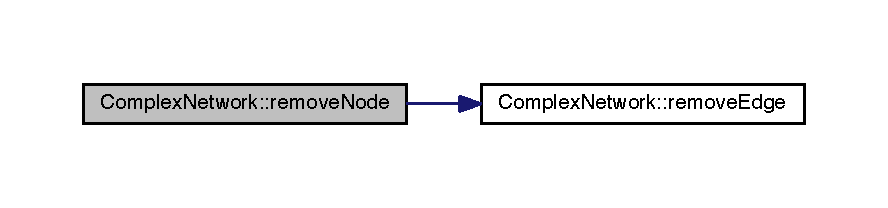
\includegraphics[width=350pt]{class_complex_network_a33f2b4528cc31296ede98be7e6dcd600_cgraph}
\end{center}
\end{figure}




Here is the caller graph for this function\+:\nopagebreak
\begin{figure}[H]
\begin{center}
\leavevmode
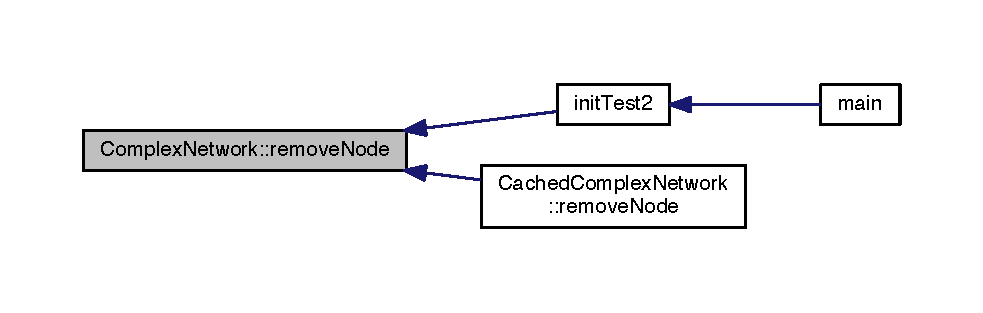
\includegraphics[width=350pt]{class_complex_network_a33f2b4528cc31296ede98be7e6dcd600_icgraph}
\end{center}
\end{figure}


\hypertarget{class_complex_network_a5d127d4296808b7ccdadccaa58084e96}{\index{Complex\+Network@{Complex\+Network}!save@{save}}
\index{save@{save}!Complex\+Network@{Complex\+Network}}
\subsubsection[{save}]{\setlength{\rightskip}{0pt plus 5cm}template$<$typename N\+O\+D\+E\+\_\+\+T\+Y\+P\+E , typename E\+D\+G\+E\+\_\+\+T\+Y\+P\+E $>$ void {\bf Complex\+Network}$<$ N\+O\+D\+E\+\_\+\+T\+Y\+P\+E, E\+D\+G\+E\+\_\+\+T\+Y\+P\+E $>$\+::save (
\begin{DoxyParamCaption}
\item[{const char $\ast$}]{filename}
\end{DoxyParamCaption}
)}}\label{class_complex_network_a5d127d4296808b7ccdadccaa58084e96}


Here is the caller graph for this function\+:\nopagebreak
\begin{figure}[H]
\begin{center}
\leavevmode
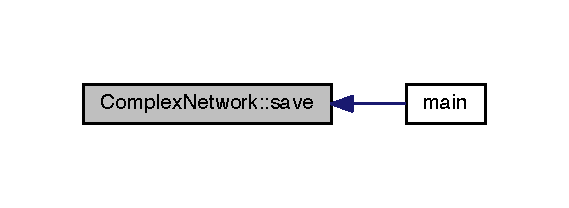
\includegraphics[width=273pt]{class_complex_network_a5d127d4296808b7ccdadccaa58084e96_icgraph}
\end{center}
\end{figure}




\subsection{Member Data Documentation}
\hypertarget{class_complex_network_a5305dba65a6d949064e46a6729c39e53}{\index{Complex\+Network@{Complex\+Network}!current\+\_\+edge\+\_\+id@{current\+\_\+edge\+\_\+id}}
\index{current\+\_\+edge\+\_\+id@{current\+\_\+edge\+\_\+id}!Complex\+Network@{Complex\+Network}}
\subsubsection[{current\+\_\+edge\+\_\+id}]{\setlength{\rightskip}{0pt plus 5cm}template$<$typename N\+O\+D\+E\+\_\+\+T\+Y\+P\+E, typename E\+D\+G\+E\+\_\+\+T\+Y\+P\+E$>$ {\bf edge\+\_\+id} {\bf Complex\+Network}$<$ N\+O\+D\+E\+\_\+\+T\+Y\+P\+E, E\+D\+G\+E\+\_\+\+T\+Y\+P\+E $>$\+::current\+\_\+edge\+\_\+id\hspace{0.3cm}{\ttfamily [protected]}}}\label{class_complex_network_a5305dba65a6d949064e46a6729c39e53}
\hypertarget{class_complex_network_ab71dc127e36a989049df28f58f2c315a}{\index{Complex\+Network@{Complex\+Network}!current\+\_\+node\+\_\+id@{current\+\_\+node\+\_\+id}}
\index{current\+\_\+node\+\_\+id@{current\+\_\+node\+\_\+id}!Complex\+Network@{Complex\+Network}}
\subsubsection[{current\+\_\+node\+\_\+id}]{\setlength{\rightskip}{0pt plus 5cm}template$<$typename N\+O\+D\+E\+\_\+\+T\+Y\+P\+E, typename E\+D\+G\+E\+\_\+\+T\+Y\+P\+E$>$ {\bf node\+\_\+id} {\bf Complex\+Network}$<$ N\+O\+D\+E\+\_\+\+T\+Y\+P\+E, E\+D\+G\+E\+\_\+\+T\+Y\+P\+E $>$\+::current\+\_\+node\+\_\+id\hspace{0.3cm}{\ttfamily [protected]}}}\label{class_complex_network_ab71dc127e36a989049df28f58f2c315a}
\hypertarget{class_complex_network_abc2c2def62701d56ec56c8b0accbedb9}{\index{Complex\+Network@{Complex\+Network}!description@{description}}
\index{description@{description}!Complex\+Network@{Complex\+Network}}
\subsubsection[{description}]{\setlength{\rightskip}{0pt plus 5cm}template$<$typename N\+O\+D\+E\+\_\+\+T\+Y\+P\+E, typename E\+D\+G\+E\+\_\+\+T\+Y\+P\+E$>$ char {\bf Complex\+Network}$<$ N\+O\+D\+E\+\_\+\+T\+Y\+P\+E, E\+D\+G\+E\+\_\+\+T\+Y\+P\+E $>$\+::description\mbox{[}200\mbox{]}}}\label{class_complex_network_abc2c2def62701d56ec56c8b0accbedb9}
\hypertarget{class_complex_network_ae1f8a32f89d84aab42475d8fe46dfa09}{\index{Complex\+Network@{Complex\+Network}!directed@{directed}}
\index{directed@{directed}!Complex\+Network@{Complex\+Network}}
\subsubsection[{directed}]{\setlength{\rightskip}{0pt plus 5cm}template$<$typename N\+O\+D\+E\+\_\+\+T\+Y\+P\+E, typename E\+D\+G\+E\+\_\+\+T\+Y\+P\+E$>$ bool {\bf Complex\+Network}$<$ N\+O\+D\+E\+\_\+\+T\+Y\+P\+E, E\+D\+G\+E\+\_\+\+T\+Y\+P\+E $>$\+::directed\hspace{0.3cm}{\ttfamily [protected]}}}\label{class_complex_network_ae1f8a32f89d84aab42475d8fe46dfa09}
\hypertarget{class_complex_network_a666bb7ad7f5ab90416f037aeb1ba11d0}{\index{Complex\+Network@{Complex\+Network}!edge@{edge}}
\index{edge@{edge}!Complex\+Network@{Complex\+Network}}
\subsubsection[{edge}]{\setlength{\rightskip}{0pt plus 5cm}template$<$typename N\+O\+D\+E\+\_\+\+T\+Y\+P\+E, typename E\+D\+G\+E\+\_\+\+T\+Y\+P\+E$>$ Q\+Hash$<$ {\bf edge\+\_\+id}, E\+D\+G\+E\+\_\+\+T\+Y\+P\+E$>$ {\bf Complex\+Network}$<$ N\+O\+D\+E\+\_\+\+T\+Y\+P\+E, E\+D\+G\+E\+\_\+\+T\+Y\+P\+E $>$\+::edge\hspace{0.3cm}{\ttfamily [protected]}}}\label{class_complex_network_a666bb7ad7f5ab90416f037aeb1ba11d0}
\hypertarget{class_complex_network_adbdf613ffde926399cd5f6e7b8c09536}{\index{Complex\+Network@{Complex\+Network}!edges@{edges}}
\index{edges@{edges}!Complex\+Network@{Complex\+Network}}
\subsubsection[{edges}]{\setlength{\rightskip}{0pt plus 5cm}template$<$typename N\+O\+D\+E\+\_\+\+T\+Y\+P\+E, typename E\+D\+G\+E\+\_\+\+T\+Y\+P\+E$>$ Q\+Hash$<$ {\bf node\+\_\+id}, Q\+Hash$<${\bf node\+\_\+id}, {\bf edge\+\_\+id}$>$ $>$ {\bf Complex\+Network}$<$ N\+O\+D\+E\+\_\+\+T\+Y\+P\+E, E\+D\+G\+E\+\_\+\+T\+Y\+P\+E $>$\+::edges\hspace{0.3cm}{\ttfamily [protected]}}}\label{class_complex_network_adbdf613ffde926399cd5f6e7b8c09536}
\hypertarget{class_complex_network_ab9ab3dbbbcd8dd173ec40938391c0fc4}{\index{Complex\+Network@{Complex\+Network}!file\+\_\+header@{file\+\_\+header}}
\index{file\+\_\+header@{file\+\_\+header}!Complex\+Network@{Complex\+Network}}
\subsubsection[{file\+\_\+header}]{\setlength{\rightskip}{0pt plus 5cm}struct \{ ... \}  {\bf Complex\+Network}$<$ N\+O\+D\+E\+\_\+\+T\+Y\+P\+E, E\+D\+G\+E\+\_\+\+T\+Y\+P\+E $>$\+::file\+\_\+header\hspace{0.3cm}{\ttfamily [protected]}}}\label{class_complex_network_ab9ab3dbbbcd8dd173ec40938391c0fc4}
\hypertarget{class_complex_network_a6b0ecc57af689b9ba9f8855132d1c275}{\index{Complex\+Network@{Complex\+Network}!nodes@{nodes}}
\index{nodes@{nodes}!Complex\+Network@{Complex\+Network}}
\subsubsection[{nodes}]{\setlength{\rightskip}{0pt plus 5cm}template$<$typename N\+O\+D\+E\+\_\+\+T\+Y\+P\+E, typename E\+D\+G\+E\+\_\+\+T\+Y\+P\+E$>$ Q\+Hash$<$ {\bf node\+\_\+id}, N\+O\+D\+E\+\_\+\+T\+Y\+P\+E$>$ {\bf Complex\+Network}$<$ N\+O\+D\+E\+\_\+\+T\+Y\+P\+E, E\+D\+G\+E\+\_\+\+T\+Y\+P\+E $>$\+::nodes\hspace{0.3cm}{\ttfamily [protected]}}}\label{class_complex_network_a6b0ecc57af689b9ba9f8855132d1c275}
\hypertarget{class_complex_network_ac4a7f179af0187eb3071969642b445cc}{\index{Complex\+Network@{Complex\+Network}!num\+\_\+edges@{num\+\_\+edges}}
\index{num\+\_\+edges@{num\+\_\+edges}!Complex\+Network@{Complex\+Network}}
\subsubsection[{num\+\_\+edges}]{\setlength{\rightskip}{0pt plus 5cm}template$<$typename N\+O\+D\+E\+\_\+\+T\+Y\+P\+E, typename E\+D\+G\+E\+\_\+\+T\+Y\+P\+E$>$ unsigned int {\bf Complex\+Network}$<$ N\+O\+D\+E\+\_\+\+T\+Y\+P\+E, E\+D\+G\+E\+\_\+\+T\+Y\+P\+E $>$\+::num\+\_\+edges}}\label{class_complex_network_ac4a7f179af0187eb3071969642b445cc}
\hypertarget{class_complex_network_a6c8777ba48e68c02d2d523abe904b6b1}{\index{Complex\+Network@{Complex\+Network}!num\+\_\+nodes@{num\+\_\+nodes}}
\index{num\+\_\+nodes@{num\+\_\+nodes}!Complex\+Network@{Complex\+Network}}
\subsubsection[{num\+\_\+nodes}]{\setlength{\rightskip}{0pt plus 5cm}template$<$typename N\+O\+D\+E\+\_\+\+T\+Y\+P\+E, typename E\+D\+G\+E\+\_\+\+T\+Y\+P\+E$>$ unsigned int {\bf Complex\+Network}$<$ N\+O\+D\+E\+\_\+\+T\+Y\+P\+E, E\+D\+G\+E\+\_\+\+T\+Y\+P\+E $>$\+::num\+\_\+nodes}}\label{class_complex_network_a6c8777ba48e68c02d2d523abe904b6b1}


The documentation for this class was generated from the following file\+:\begin{DoxyCompactItemize}
\item 
Sources/\+Complex\+Network/\hyperlink{_complex_network_8hpp}{Complex\+Network.\+hpp}\end{DoxyCompactItemize}

\hypertarget{class_edge}{\section{Edge$<$ N\+O\+D\+E\+\_\+\+T\+Y\+P\+E, E\+D\+G\+E\+\_\+\+T\+Y\+P\+E $>$ Class Template Reference}
\label{class_edge}\index{Edge$<$ N\+O\+D\+E\+\_\+\+T\+Y\+P\+E, E\+D\+G\+E\+\_\+\+T\+Y\+P\+E $>$@{Edge$<$ N\+O\+D\+E\+\_\+\+T\+Y\+P\+E, E\+D\+G\+E\+\_\+\+T\+Y\+P\+E $>$}}
}


{\ttfamily \#include $<$Edge.\+hpp$>$}

\subsection*{Public Member Functions}
\begin{DoxyCompactItemize}
\item 
E\+D\+G\+E\+\_\+\+T\+Y\+P\+E \hyperlink{class_edge_a3352ae81439c772a0ebe640f14f8b910}{get\+Attribute} ()
\item 
void \hyperlink{class_edge_aa63f7fac23602924d2e19f1389a93620}{set\+Attribute} (E\+D\+G\+E\+\_\+\+T\+Y\+P\+E attr)
\item 
\hyperlink{class_edge_a16c5157732e48a737ca0a1d7841e8e19}{Edge} (\hyperlink{class_node}{Node}$<$ N\+O\+D\+E\+\_\+\+T\+Y\+P\+E, E\+D\+G\+E\+\_\+\+T\+Y\+P\+E $>$ $\ast$\hyperlink{class_edge_a1bffa41df2941b7d55c59a5031f78e14}{from}, \hyperlink{class_node}{Node}$<$ N\+O\+D\+E\+\_\+\+T\+Y\+P\+E, E\+D\+G\+E\+\_\+\+T\+Y\+P\+E $>$ $\ast$\hyperlink{class_edge_a7ba6dee1554e4a0a7cf69862e90fdd85}{to})
\item 
\hyperlink{class_edge_a6d1f57f17db61020c1e51c09ff8ab7bb}{Edge} (\hyperlink{class_node}{Node}$<$ N\+O\+D\+E\+\_\+\+T\+Y\+P\+E, E\+D\+G\+E\+\_\+\+T\+Y\+P\+E $>$ $\ast$\hyperlink{class_edge_a1bffa41df2941b7d55c59a5031f78e14}{from}, \hyperlink{class_node}{Node}$<$ N\+O\+D\+E\+\_\+\+T\+Y\+P\+E, E\+D\+G\+E\+\_\+\+T\+Y\+P\+E $>$ $\ast$\hyperlink{class_edge_a7ba6dee1554e4a0a7cf69862e90fdd85}{to}, E\+D\+G\+E\+\_\+\+T\+Y\+P\+E \hyperlink{class_edge_ae49cc056dfa848b0a1beef821d81a31d}{attribute})
\end{DoxyCompactItemize}
\subsection*{Private Attributes}
\begin{DoxyCompactItemize}
\item 
\hyperlink{class_node}{Node}$<$ N\+O\+D\+E\+\_\+\+T\+Y\+P\+E, E\+D\+G\+E\+\_\+\+T\+Y\+P\+E $>$ $\ast$ \hyperlink{class_edge_a1bffa41df2941b7d55c59a5031f78e14}{from}
\item 
\hyperlink{class_node}{Node}$<$ N\+O\+D\+E\+\_\+\+T\+Y\+P\+E, E\+D\+G\+E\+\_\+\+T\+Y\+P\+E $>$ $\ast$ \hyperlink{class_edge_a7ba6dee1554e4a0a7cf69862e90fdd85}{to}
\item 
E\+D\+G\+E\+\_\+\+T\+Y\+P\+E \hyperlink{class_edge_ae49cc056dfa848b0a1beef821d81a31d}{attribute}
\end{DoxyCompactItemize}
\subsection*{Friends}
\begin{DoxyCompactItemize}
\item 
class \hyperlink{class_edge_ad8438fc5199b628ea294f77319026b6a}{Complex\+Network$<$ N\+O\+D\+E\+\_\+\+T\+Y\+P\+E, E\+D\+G\+E\+\_\+\+T\+Y\+P\+E $>$}
\end{DoxyCompactItemize}


Collaboration diagram for Edge$<$ N\+O\+D\+E\+\_\+\+T\+Y\+P\+E, E\+D\+G\+E\+\_\+\+T\+Y\+P\+E $>$\+:\nopagebreak
\begin{figure}[H]
\begin{center}
\leavevmode
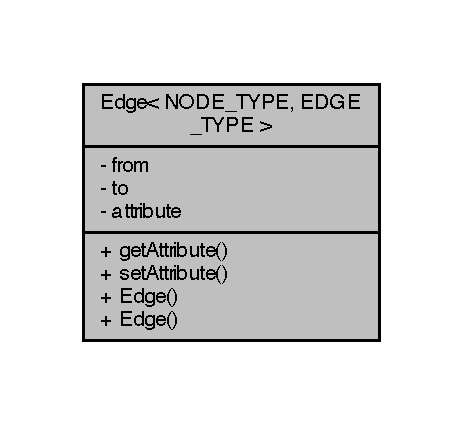
\includegraphics[width=222pt]{class_edge__coll__graph}
\end{center}
\end{figure}


\subsection{Constructor \& Destructor Documentation}
\hypertarget{class_edge_a16c5157732e48a737ca0a1d7841e8e19}{\index{Edge@{Edge}!Edge@{Edge}}
\index{Edge@{Edge}!Edge@{Edge}}
\subsubsection[{Edge}]{\setlength{\rightskip}{0pt plus 5cm}template$<$class N\+O\+D\+E\+\_\+\+T\+Y\+P\+E , class E\+D\+G\+E\+\_\+\+T\+Y\+P\+E $>$ {\bf Edge}$<$ N\+O\+D\+E\+\_\+\+T\+Y\+P\+E, E\+D\+G\+E\+\_\+\+T\+Y\+P\+E $>$\+::{\bf Edge} (
\begin{DoxyParamCaption}
\item[{{\bf Node}$<$ N\+O\+D\+E\+\_\+\+T\+Y\+P\+E, E\+D\+G\+E\+\_\+\+T\+Y\+P\+E $>$ $\ast$}]{from, }
\item[{{\bf Node}$<$ N\+O\+D\+E\+\_\+\+T\+Y\+P\+E, E\+D\+G\+E\+\_\+\+T\+Y\+P\+E $>$ $\ast$}]{to}
\end{DoxyParamCaption}
)}}\label{class_edge_a16c5157732e48a737ca0a1d7841e8e19}
Por padrão as arestas são direcionadas 
\begin{DoxyParams}{Parameters}
{\em from} & Nó de saída \\
\hline
{\em to} & Nó de entrada \\
\hline
\end{DoxyParams}
\hypertarget{class_edge_a6d1f57f17db61020c1e51c09ff8ab7bb}{\index{Edge@{Edge}!Edge@{Edge}}
\index{Edge@{Edge}!Edge@{Edge}}
\subsubsection[{Edge}]{\setlength{\rightskip}{0pt plus 5cm}template$<$class N\+O\+D\+E\+\_\+\+T\+Y\+P\+E , class E\+D\+G\+E\+\_\+\+T\+Y\+P\+E $>$ {\bf Edge}$<$ N\+O\+D\+E\+\_\+\+T\+Y\+P\+E, E\+D\+G\+E\+\_\+\+T\+Y\+P\+E $>$\+::{\bf Edge} (
\begin{DoxyParamCaption}
\item[{{\bf Node}$<$ N\+O\+D\+E\+\_\+\+T\+Y\+P\+E, E\+D\+G\+E\+\_\+\+T\+Y\+P\+E $>$ $\ast$}]{from, }
\item[{{\bf Node}$<$ N\+O\+D\+E\+\_\+\+T\+Y\+P\+E, E\+D\+G\+E\+\_\+\+T\+Y\+P\+E $>$ $\ast$}]{to, }
\item[{E\+D\+G\+E\+\_\+\+T\+Y\+P\+E}]{attribute}
\end{DoxyParamCaption}
)}}\label{class_edge_a6d1f57f17db61020c1e51c09ff8ab7bb}
Por padrão as arestas são direcionadas 
\begin{DoxyParams}{Parameters}
{\em from} & Nó de saída \\
\hline
{\em to} & Nó de entrada \\
\hline
{\em attribute} & Atributo da aresta \\
\hline
\end{DoxyParams}


\subsection{Member Function Documentation}
\hypertarget{class_edge_a3352ae81439c772a0ebe640f14f8b910}{\index{Edge@{Edge}!get\+Attribute@{get\+Attribute}}
\index{get\+Attribute@{get\+Attribute}!Edge@{Edge}}
\subsubsection[{get\+Attribute}]{\setlength{\rightskip}{0pt plus 5cm}template$<$class N\+O\+D\+E\+\_\+\+T\+Y\+P\+E , class E\+D\+G\+E\+\_\+\+T\+Y\+P\+E $>$ E\+D\+G\+E\+\_\+\+T\+Y\+P\+E {\bf Edge}$<$ N\+O\+D\+E\+\_\+\+T\+Y\+P\+E, E\+D\+G\+E\+\_\+\+T\+Y\+P\+E $>$\+::get\+Attribute (
\begin{DoxyParamCaption}
{}
\end{DoxyParamCaption}
)}}\label{class_edge_a3352ae81439c772a0ebe640f14f8b910}


Here is the caller graph for this function\+:\nopagebreak
\begin{figure}[H]
\begin{center}
\leavevmode
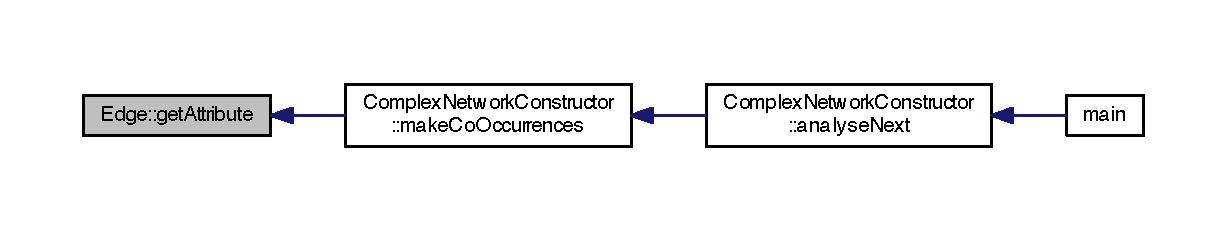
\includegraphics[width=350pt]{class_edge_a3352ae81439c772a0ebe640f14f8b910_icgraph}
\end{center}
\end{figure}


\hypertarget{class_edge_aa63f7fac23602924d2e19f1389a93620}{\index{Edge@{Edge}!set\+Attribute@{set\+Attribute}}
\index{set\+Attribute@{set\+Attribute}!Edge@{Edge}}
\subsubsection[{set\+Attribute}]{\setlength{\rightskip}{0pt plus 5cm}template$<$class N\+O\+D\+E\+\_\+\+T\+Y\+P\+E , class E\+D\+G\+E\+\_\+\+T\+Y\+P\+E $>$ void {\bf Edge}$<$ N\+O\+D\+E\+\_\+\+T\+Y\+P\+E, E\+D\+G\+E\+\_\+\+T\+Y\+P\+E $>$\+::set\+Attribute (
\begin{DoxyParamCaption}
\item[{E\+D\+G\+E\+\_\+\+T\+Y\+P\+E}]{attr}
\end{DoxyParamCaption}
)}}\label{class_edge_aa63f7fac23602924d2e19f1389a93620}


Here is the caller graph for this function\+:\nopagebreak
\begin{figure}[H]
\begin{center}
\leavevmode
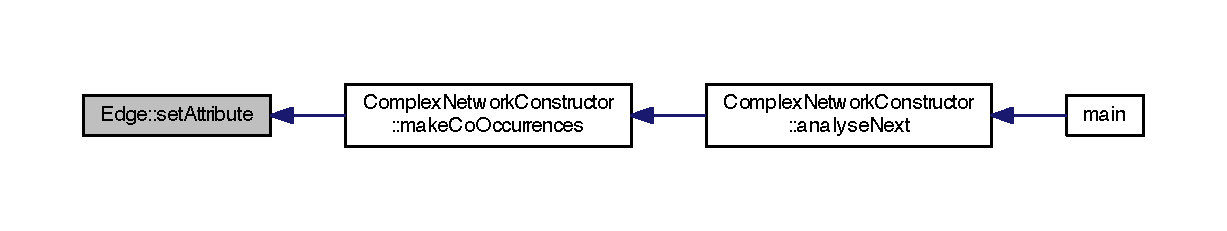
\includegraphics[width=350pt]{class_edge_aa63f7fac23602924d2e19f1389a93620_icgraph}
\end{center}
\end{figure}




\subsection{Friends And Related Function Documentation}
\hypertarget{class_edge_ad8438fc5199b628ea294f77319026b6a}{\index{Edge@{Edge}!Complex\+Network$<$ N\+O\+D\+E\+\_\+\+T\+Y\+P\+E, E\+D\+G\+E\+\_\+\+T\+Y\+P\+E $>$@{Complex\+Network$<$ N\+O\+D\+E\+\_\+\+T\+Y\+P\+E, E\+D\+G\+E\+\_\+\+T\+Y\+P\+E $>$}}
\index{Complex\+Network$<$ N\+O\+D\+E\+\_\+\+T\+Y\+P\+E, E\+D\+G\+E\+\_\+\+T\+Y\+P\+E $>$@{Complex\+Network$<$ N\+O\+D\+E\+\_\+\+T\+Y\+P\+E, E\+D\+G\+E\+\_\+\+T\+Y\+P\+E $>$}!Edge@{Edge}}
\subsubsection[{Complex\+Network$<$ N\+O\+D\+E\+\_\+\+T\+Y\+P\+E, E\+D\+G\+E\+\_\+\+T\+Y\+P\+E $>$}]{\setlength{\rightskip}{0pt plus 5cm}template$<$class N\+O\+D\+E\+\_\+\+T\+Y\+P\+E, class E\+D\+G\+E\+\_\+\+T\+Y\+P\+E$>$ friend class {\bf Complex\+Network}$<$ N\+O\+D\+E\+\_\+\+T\+Y\+P\+E, E\+D\+G\+E\+\_\+\+T\+Y\+P\+E $>$\hspace{0.3cm}{\ttfamily [friend]}}}\label{class_edge_ad8438fc5199b628ea294f77319026b6a}


\subsection{Member Data Documentation}
\hypertarget{class_edge_ae49cc056dfa848b0a1beef821d81a31d}{\index{Edge@{Edge}!attribute@{attribute}}
\index{attribute@{attribute}!Edge@{Edge}}
\subsubsection[{attribute}]{\setlength{\rightskip}{0pt plus 5cm}template$<$class N\+O\+D\+E\+\_\+\+T\+Y\+P\+E, class E\+D\+G\+E\+\_\+\+T\+Y\+P\+E$>$ E\+D\+G\+E\+\_\+\+T\+Y\+P\+E {\bf Edge}$<$ N\+O\+D\+E\+\_\+\+T\+Y\+P\+E, E\+D\+G\+E\+\_\+\+T\+Y\+P\+E $>$\+::attribute\hspace{0.3cm}{\ttfamily [private]}}}\label{class_edge_ae49cc056dfa848b0a1beef821d81a31d}
\hypertarget{class_edge_a1bffa41df2941b7d55c59a5031f78e14}{\index{Edge@{Edge}!from@{from}}
\index{from@{from}!Edge@{Edge}}
\subsubsection[{from}]{\setlength{\rightskip}{0pt plus 5cm}template$<$class N\+O\+D\+E\+\_\+\+T\+Y\+P\+E, class E\+D\+G\+E\+\_\+\+T\+Y\+P\+E$>$ {\bf Node}$<$N\+O\+D\+E\+\_\+\+T\+Y\+P\+E, E\+D\+G\+E\+\_\+\+T\+Y\+P\+E$>$$\ast$ {\bf Edge}$<$ N\+O\+D\+E\+\_\+\+T\+Y\+P\+E, E\+D\+G\+E\+\_\+\+T\+Y\+P\+E $>$\+::from\hspace{0.3cm}{\ttfamily [private]}}}\label{class_edge_a1bffa41df2941b7d55c59a5031f78e14}
\hypertarget{class_edge_a7ba6dee1554e4a0a7cf69862e90fdd85}{\index{Edge@{Edge}!to@{to}}
\index{to@{to}!Edge@{Edge}}
\subsubsection[{to}]{\setlength{\rightskip}{0pt plus 5cm}template$<$class N\+O\+D\+E\+\_\+\+T\+Y\+P\+E, class E\+D\+G\+E\+\_\+\+T\+Y\+P\+E$>$ {\bf Node}$<$N\+O\+D\+E\+\_\+\+T\+Y\+P\+E, E\+D\+G\+E\+\_\+\+T\+Y\+P\+E$>$$\ast$ {\bf Edge}$<$ N\+O\+D\+E\+\_\+\+T\+Y\+P\+E, E\+D\+G\+E\+\_\+\+T\+Y\+P\+E $>$\+::to\hspace{0.3cm}{\ttfamily [private]}}}\label{class_edge_a7ba6dee1554e4a0a7cf69862e90fdd85}


The documentation for this class was generated from the following file\+:\begin{DoxyCompactItemize}
\item 
src/\hyperlink{_edge_8hpp}{Edge.\+hpp}\end{DoxyCompactItemize}

\hypertarget{class_node}{\section{Node$<$ N\+O\+D\+E\+\_\+\+T\+Y\+P\+E, E\+D\+G\+E\+\_\+\+T\+Y\+P\+E $>$ Class Template Reference}
\label{class_node}\index{Node$<$ N\+O\+D\+E\+\_\+\+T\+Y\+P\+E, E\+D\+G\+E\+\_\+\+T\+Y\+P\+E $>$@{Node$<$ N\+O\+D\+E\+\_\+\+T\+Y\+P\+E, E\+D\+G\+E\+\_\+\+T\+Y\+P\+E $>$}}
}


{\ttfamily \#include $<$Node.\+hpp$>$}



Collaboration diagram for Node$<$ N\+O\+D\+E\+\_\+\+T\+Y\+P\+E, E\+D\+G\+E\+\_\+\+T\+Y\+P\+E $>$\+:
\nopagebreak
\begin{figure}[H]
\begin{center}
\leavevmode
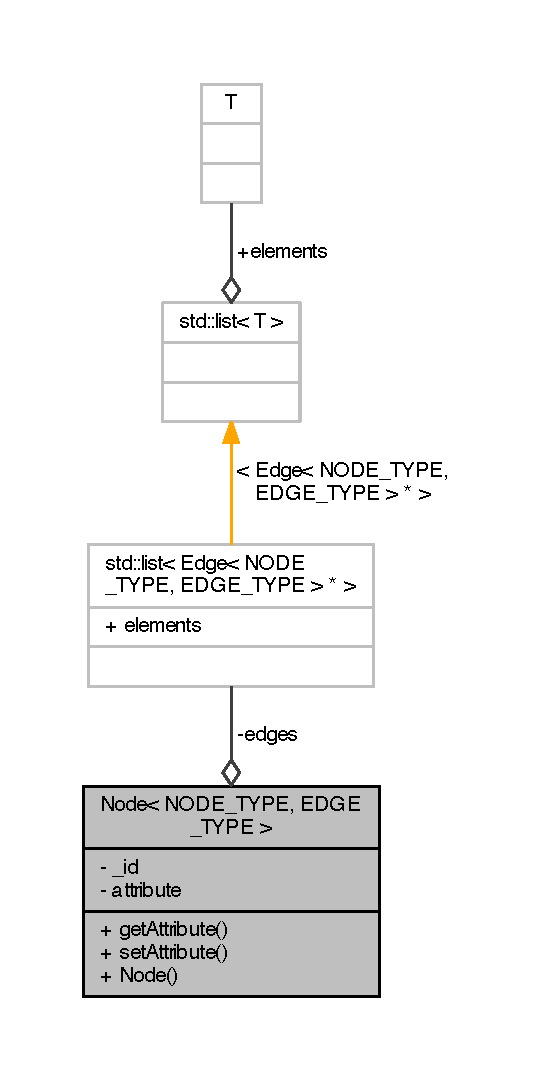
\includegraphics[width=222pt]{class_node__coll__graph}
\end{center}
\end{figure}
\subsection*{Public Member Functions}
\begin{DoxyCompactItemize}
\item 
N\+O\+D\+E\+\_\+\+T\+Y\+P\+E \hyperlink{class_node_a1272270025389e601164431b42ab5237}{get\+Attribute} ()
\item 
void \hyperlink{class_node_acb8f913ce2f995a6a14b9b05c60938f8}{set\+Attribute} (N\+O\+D\+E\+\_\+\+T\+Y\+P\+E attr)
\item 
\hyperlink{class_node_a94263af6c10cc9882d33918080dc722f}{Node} (N\+O\+D\+E\+\_\+\+T\+Y\+P\+E \hyperlink{class_node_a434cad0f70931bc3aaa048d52d0b0ee3}{attribute})
\end{DoxyCompactItemize}
\subsection*{Private Attributes}
\begin{DoxyCompactItemize}
\item 
int \hyperlink{class_node_a533ab17912d5b919a37ada31a8a78dc4}{\+\_\+id}
\item 
N\+O\+D\+E\+\_\+\+T\+Y\+P\+E \hyperlink{class_node_a434cad0f70931bc3aaa048d52d0b0ee3}{attribute}
\end{DoxyCompactItemize}


\subsection{Constructor \& Destructor Documentation}
\hypertarget{class_node_a94263af6c10cc9882d33918080dc722f}{\index{Node@{Node}!Node@{Node}}
\index{Node@{Node}!Node@{Node}}
\subsubsection[{Node}]{\setlength{\rightskip}{0pt plus 5cm}template$<$class N\+O\+D\+E\+\_\+\+T\+Y\+P\+E , class E\+D\+G\+E\+\_\+\+T\+Y\+P\+E $>$ {\bf Node}$<$ N\+O\+D\+E\+\_\+\+T\+Y\+P\+E, E\+D\+G\+E\+\_\+\+T\+Y\+P\+E $>$\+::{\bf Node} (
\begin{DoxyParamCaption}
\item[{N\+O\+D\+E\+\_\+\+T\+Y\+P\+E}]{attribute}
\end{DoxyParamCaption}
)}}\label{class_node_a94263af6c10cc9882d33918080dc722f}


\subsection{Member Function Documentation}
\hypertarget{class_node_a1272270025389e601164431b42ab5237}{\index{Node@{Node}!get\+Attribute@{get\+Attribute}}
\index{get\+Attribute@{get\+Attribute}!Node@{Node}}
\subsubsection[{get\+Attribute}]{\setlength{\rightskip}{0pt plus 5cm}template$<$class N\+O\+D\+E\+\_\+\+T\+Y\+P\+E , class E\+D\+G\+E\+\_\+\+T\+Y\+P\+E $>$ N\+O\+D\+E\+\_\+\+T\+Y\+P\+E {\bf Node}$<$ N\+O\+D\+E\+\_\+\+T\+Y\+P\+E, E\+D\+G\+E\+\_\+\+T\+Y\+P\+E $>$\+::get\+Attribute (
\begin{DoxyParamCaption}
{}
\end{DoxyParamCaption}
)}}\label{class_node_a1272270025389e601164431b42ab5237}


Here is the caller graph for this function\+:
\nopagebreak
\begin{figure}[H]
\begin{center}
\leavevmode
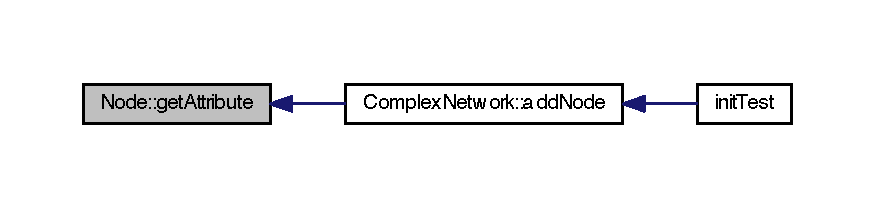
\includegraphics[width=350pt]{class_node_a1272270025389e601164431b42ab5237_icgraph}
\end{center}
\end{figure}


\hypertarget{class_node_acb8f913ce2f995a6a14b9b05c60938f8}{\index{Node@{Node}!set\+Attribute@{set\+Attribute}}
\index{set\+Attribute@{set\+Attribute}!Node@{Node}}
\subsubsection[{set\+Attribute}]{\setlength{\rightskip}{0pt plus 5cm}template$<$class N\+O\+D\+E\+\_\+\+T\+Y\+P\+E , class E\+D\+G\+E\+\_\+\+T\+Y\+P\+E $>$ void {\bf Node}$<$ N\+O\+D\+E\+\_\+\+T\+Y\+P\+E, E\+D\+G\+E\+\_\+\+T\+Y\+P\+E $>$\+::set\+Attribute (
\begin{DoxyParamCaption}
\item[{N\+O\+D\+E\+\_\+\+T\+Y\+P\+E}]{attr}
\end{DoxyParamCaption}
)}}\label{class_node_acb8f913ce2f995a6a14b9b05c60938f8}


\subsection{Member Data Documentation}
\hypertarget{class_node_a533ab17912d5b919a37ada31a8a78dc4}{\index{Node@{Node}!\+\_\+id@{\+\_\+id}}
\index{\+\_\+id@{\+\_\+id}!Node@{Node}}
\subsubsection[{\+\_\+id}]{\setlength{\rightskip}{0pt plus 5cm}template$<$class N\+O\+D\+E\+\_\+\+T\+Y\+P\+E, class E\+D\+G\+E\+\_\+\+T\+Y\+P\+E$>$ int {\bf Node}$<$ N\+O\+D\+E\+\_\+\+T\+Y\+P\+E, E\+D\+G\+E\+\_\+\+T\+Y\+P\+E $>$\+::\+\_\+id\hspace{0.3cm}{\ttfamily [private]}}}\label{class_node_a533ab17912d5b919a37ada31a8a78dc4}
\hypertarget{class_node_a434cad0f70931bc3aaa048d52d0b0ee3}{\index{Node@{Node}!attribute@{attribute}}
\index{attribute@{attribute}!Node@{Node}}
\subsubsection[{attribute}]{\setlength{\rightskip}{0pt plus 5cm}template$<$class N\+O\+D\+E\+\_\+\+T\+Y\+P\+E, class E\+D\+G\+E\+\_\+\+T\+Y\+P\+E$>$ N\+O\+D\+E\+\_\+\+T\+Y\+P\+E {\bf Node}$<$ N\+O\+D\+E\+\_\+\+T\+Y\+P\+E, E\+D\+G\+E\+\_\+\+T\+Y\+P\+E $>$\+::attribute\hspace{0.3cm}{\ttfamily [private]}}}\label{class_node_a434cad0f70931bc3aaa048d52d0b0ee3}


The documentation for this class was generated from the following file\+:\begin{DoxyCompactItemize}
\item 
src/\hyperlink{_node_8hpp}{Node.\+hpp}\end{DoxyCompactItemize}

\chapter{File Documentation}
\hypertarget{_complex_network_8cpp}{\section{Sources/\+Complex\+Network/\+Complex\+Network.cpp File Reference}
\label{_complex_network_8cpp}\index{Sources/\+Complex\+Network/\+Complex\+Network.\+cpp@{Sources/\+Complex\+Network/\+Complex\+Network.\+cpp}}
}
{\ttfamily \#include \char`\"{}Complex\+Network.\+hpp\char`\"{}}\\*
Include dependency graph for Complex\+Network.\+cpp\+:\nopagebreak
\begin{figure}[H]
\begin{center}
\leavevmode
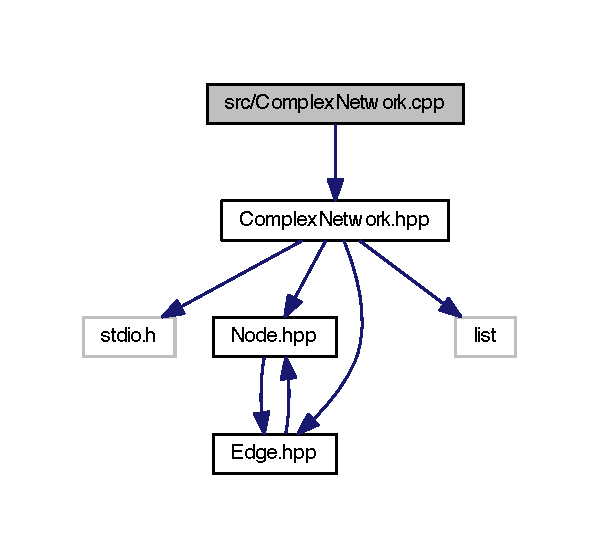
\includegraphics[width=248pt]{_complex_network_8cpp__incl}
\end{center}
\end{figure}

\hypertarget{_complex_network_8hpp}{\section{src/\+Complex\+Network.hpp File Reference}
\label{_complex_network_8hpp}\index{src/\+Complex\+Network.\+hpp@{src/\+Complex\+Network.\+hpp}}
}
{\ttfamily \#include $<$stdio.\+h$>$}\\*
{\ttfamily \#include \char`\"{}Node.\+hpp\char`\"{}}\\*
{\ttfamily \#include \char`\"{}Edge.\+hpp\char`\"{}}\\*
{\ttfamily \#include $<$list$>$}\\*
{\ttfamily \#include $<$algorithm$>$}\\*
{\ttfamily \#include $<$map$>$}\\*
Include dependency graph for Complex\+Network.\+hpp\+:\nopagebreak
\begin{figure}[H]
\begin{center}
\leavevmode
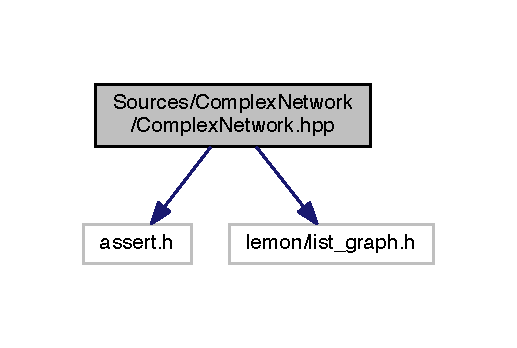
\includegraphics[width=350pt]{_complex_network_8hpp__incl}
\end{center}
\end{figure}
This graph shows which files directly or indirectly include this file\+:
\nopagebreak
\begin{figure}[H]
\begin{center}
\leavevmode
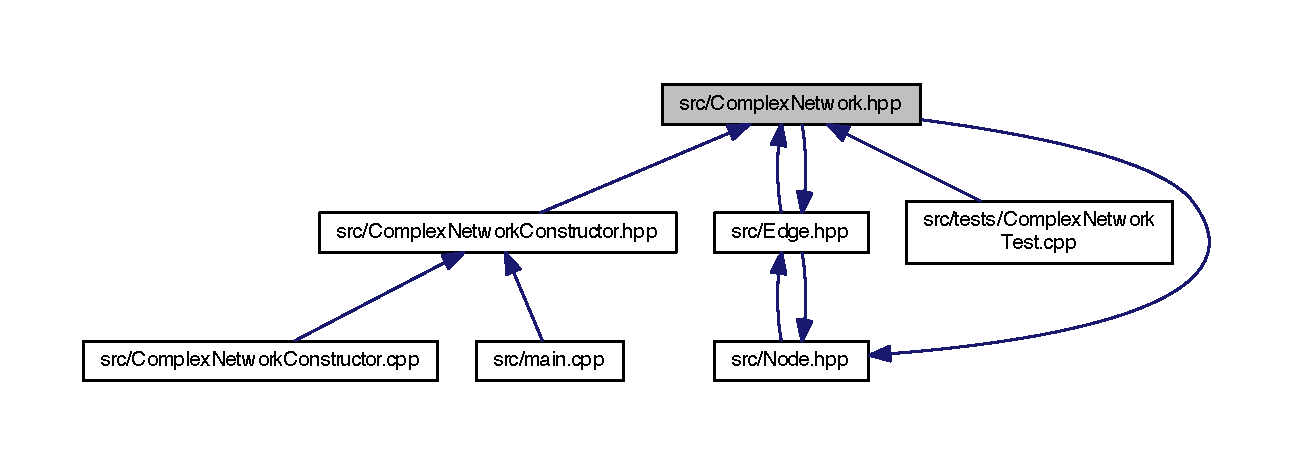
\includegraphics[width=350pt]{_complex_network_8hpp__dep__incl}
\end{center}
\end{figure}
\subsection*{Classes}
\begin{DoxyCompactItemize}
\item 
class \hyperlink{class_complex_network}{Complex\+Network$<$ N\+O\+D\+E\+\_\+\+T\+Y\+P\+E, E\+D\+G\+E\+\_\+\+T\+Y\+P\+E $>$}
\begin{DoxyCompactList}\small\item\em Rede Complexa. \end{DoxyCompactList}\end{DoxyCompactItemize}

\hypertarget{_edge_8cpp}{\section{src/\+Edge.cpp File Reference}
\label{_edge_8cpp}\index{src/\+Edge.\+cpp@{src/\+Edge.\+cpp}}
}
{\ttfamily \#include \char`\"{}Edge.\+hpp\char`\"{}}\\*
Include dependency graph for Edge.\+cpp\+:\nopagebreak
\begin{figure}[H]
\begin{center}
\leavevmode
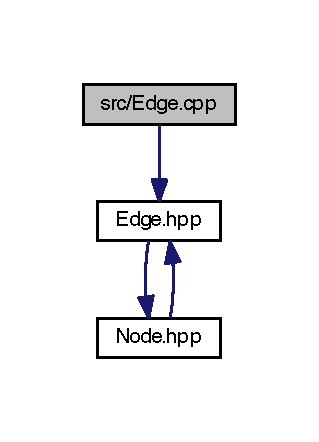
\includegraphics[width=153pt]{_edge_8cpp__incl}
\end{center}
\end{figure}

\hypertarget{_edge_8hpp}{\section{src/\+Edge.hpp File Reference}
\label{_edge_8hpp}\index{src/\+Edge.\+hpp@{src/\+Edge.\+hpp}}
}
{\ttfamily \#include \char`\"{}Node.\+hpp\char`\"{}}\\*
Include dependency graph for Edge.\+hpp\+:\nopagebreak
\begin{figure}[H]
\begin{center}
\leavevmode
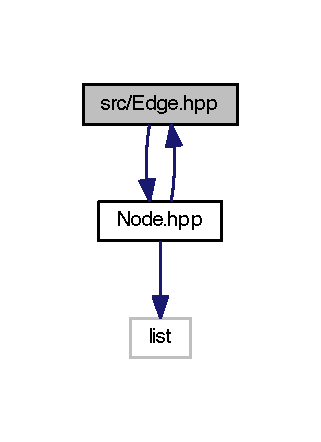
\includegraphics[width=154pt]{_edge_8hpp__incl}
\end{center}
\end{figure}
This graph shows which files directly or indirectly include this file\+:\nopagebreak
\begin{figure}[H]
\begin{center}
\leavevmode
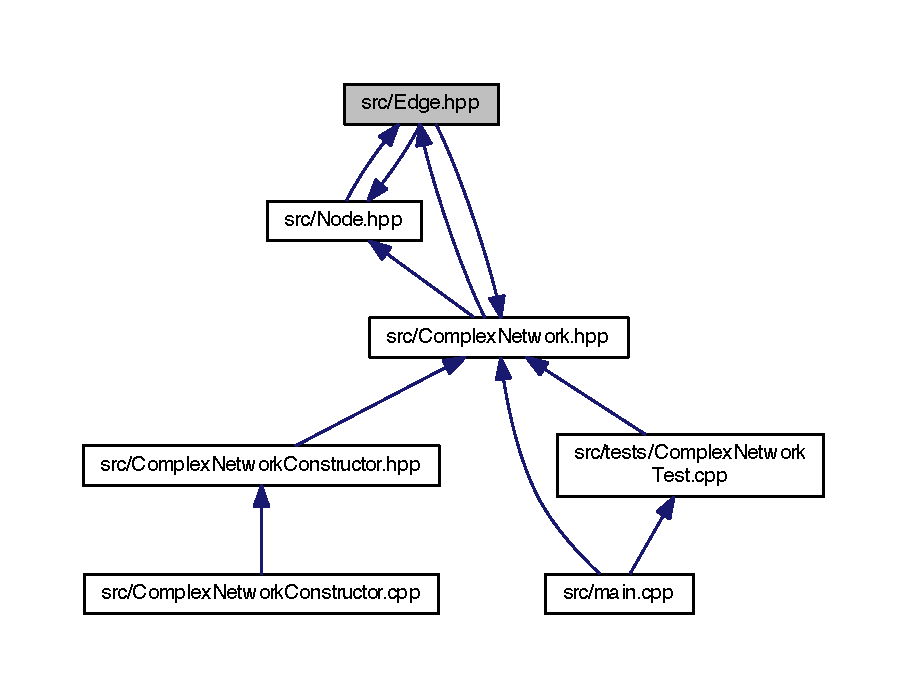
\includegraphics[width=350pt]{_edge_8hpp__dep__incl}
\end{center}
\end{figure}
\subsection*{Classes}
\begin{DoxyCompactItemize}
\item 
class \hyperlink{class_edge}{Edge$<$ A\+T\+T\+R\+\_\+\+T\+Y\+P\+E, N\+O\+D\+E\+\_\+\+T\+Y\+P\+E $>$}
\item 
class \hyperlink{class_edge}{Edge$<$ A\+T\+T\+R\+\_\+\+T\+Y\+P\+E, N\+O\+D\+E\+\_\+\+T\+Y\+P\+E $>$}
\end{DoxyCompactItemize}

\hypertarget{main_8cpp}{\section{src/main.cpp File Reference}
\label{main_8cpp}\index{src/main.\+cpp@{src/main.\+cpp}}
}
{\ttfamily \#include $<$stdio.\+h$>$}\\*
{\ttfamily \#include $<$Q\+Application$>$}\\*
{\ttfamily \#include \char`\"{}Complex\+Network.\+hpp\char`\"{}}\\*
{\ttfamily \#include \char`\"{}tests/\+Complex\+Network\+Test.\+cpp\char`\"{}}\\*
{\ttfamily \#include \char`\"{}Sun\+Database\+Reader.\+hpp\char`\"{}}\\*
{\ttfamily \#include \char`\"{}Area\+Feature.\+hpp\char`\"{}}\\*
{\ttfamily \#include $<$locale$>$}\\*
Include dependency graph for main.\+cpp\+:
\nopagebreak
\begin{figure}[H]
\begin{center}
\leavevmode
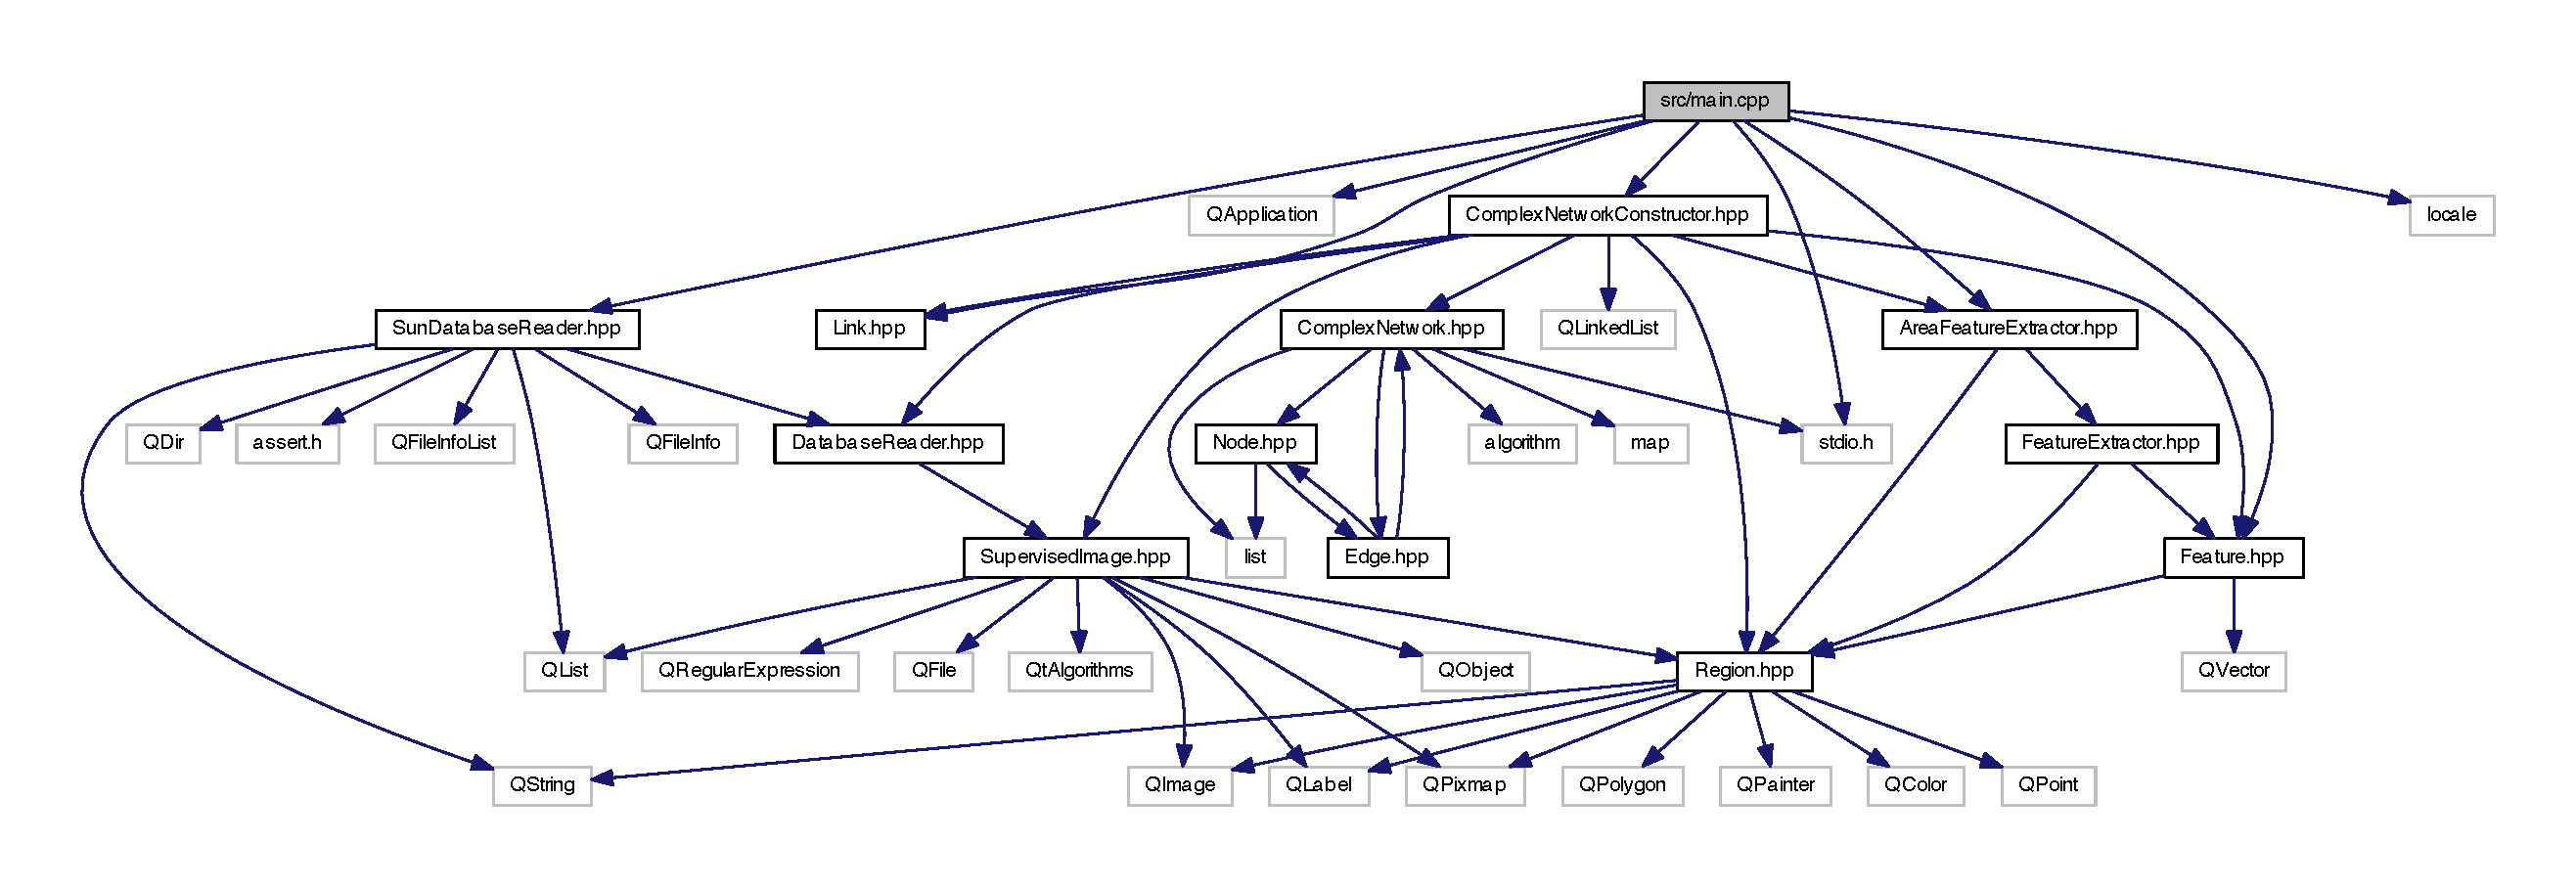
\includegraphics[width=350pt]{main_8cpp__incl}
\end{center}
\end{figure}
\subsection*{Functions}
\begin{DoxyCompactItemize}
\item 
int \hyperlink{main_8cpp_a3c04138a5bfe5d72780bb7e82a18e627}{main} (int argc, char $\ast$$\ast$argv)
\end{DoxyCompactItemize}


\subsection{Function Documentation}
\hypertarget{main_8cpp_a3c04138a5bfe5d72780bb7e82a18e627}{\index{main.\+cpp@{main.\+cpp}!main@{main}}
\index{main@{main}!main.\+cpp@{main.\+cpp}}
\subsubsection[{main}]{\setlength{\rightskip}{0pt plus 5cm}int main (
\begin{DoxyParamCaption}
\item[{int}]{argc, }
\item[{char $\ast$$\ast$}]{argv}
\end{DoxyParamCaption}
)}}\label{main_8cpp_a3c04138a5bfe5d72780bb7e82a18e627}


Here is the call graph for this function\+:
\nopagebreak
\begin{figure}[H]
\begin{center}
\leavevmode
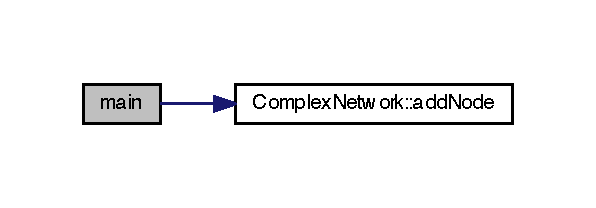
\includegraphics[width=350pt]{main_8cpp_a3c04138a5bfe5d72780bb7e82a18e627_cgraph}
\end{center}
\end{figure}



\hypertarget{_node_8cpp}{\section{src/\+Node.cpp File Reference}
\label{_node_8cpp}\index{src/\+Node.\+cpp@{src/\+Node.\+cpp}}
}
{\ttfamily \#include \char`\"{}Node.\+hpp\char`\"{}}\\*
Include dependency graph for Node.\+cpp\+:\nopagebreak
\begin{figure}[H]
\begin{center}
\leavevmode
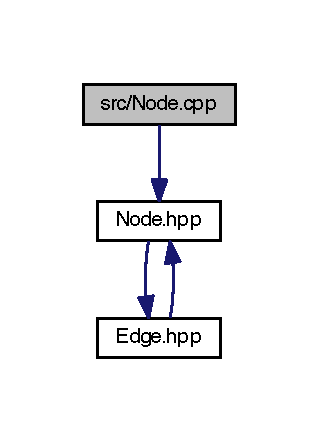
\includegraphics[width=153pt]{_node_8cpp__incl}
\end{center}
\end{figure}

\hypertarget{_node_8hpp}{\section{src/\+Node.hpp File Reference}
\label{_node_8hpp}\index{src/\+Node.\+hpp@{src/\+Node.\+hpp}}
}
{\ttfamily \#include \char`\"{}Edge.\+hpp\char`\"{}}\\*
{\ttfamily \#include $<$list$>$}\\*
Include dependency graph for Node.\+hpp\+:\nopagebreak
\begin{figure}[H]
\begin{center}
\leavevmode
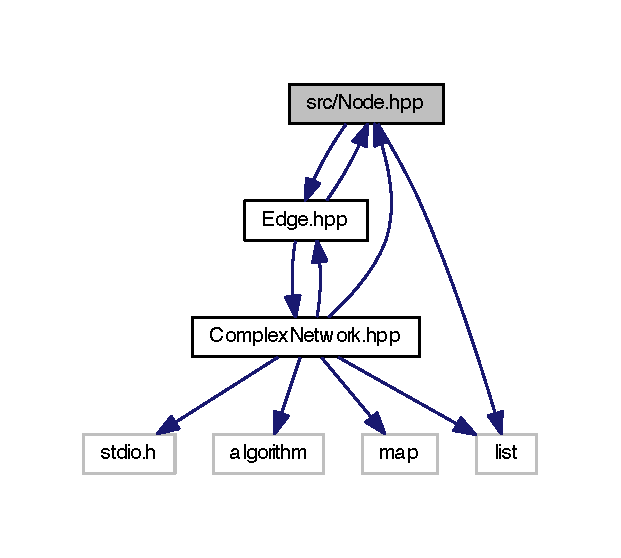
\includegraphics[width=194pt]{_node_8hpp__incl}
\end{center}
\end{figure}
This graph shows which files directly or indirectly include this file\+:\nopagebreak
\begin{figure}[H]
\begin{center}
\leavevmode
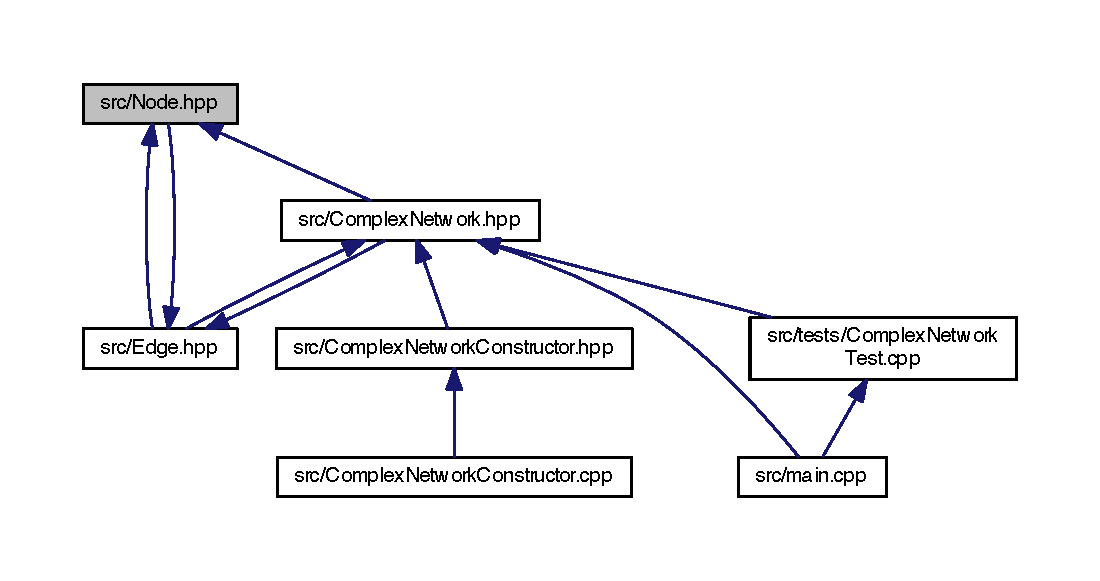
\includegraphics[width=212pt]{_node_8hpp__dep__incl}
\end{center}
\end{figure}
\subsection*{Classes}
\begin{DoxyCompactItemize}
\item 
class \hyperlink{class_node}{Node$<$ N\+O\+D\+E\+\_\+\+T\+Y\+P\+E, E\+D\+G\+E\+\_\+\+T\+Y\+P\+E $>$}
\item 
class \hyperlink{class_node}{Node$<$ N\+O\+D\+E\+\_\+\+T\+Y\+P\+E, E\+D\+G\+E\+\_\+\+T\+Y\+P\+E $>$}
\end{DoxyCompactItemize}

%--- End generated contents ---

% Index
\newpage
\phantomsection
\addcontentsline{toc}{chapter}{Index}
\printindex

\end{document}
